\documentclass[toc=sectionentrywithdots,a4paper,12pt,oneside]{scrartcl}
%\documentclass[toc=sectionentrywithdots,a4paper,11pt,oneside,openright]{scrartcl}

% Stilistische Vorgaben nach Standard der HS
%--------------------------------------------------------------------------
\usepackage{geometry}
\geometry{top=2.0cm,bottom=3cm,left=3.5cm,right=2cm}
%----------------Schriftart/-form------------------
%Serifen######
%-------------
%\usepackage{mathptmx} % setzt auf Times New Roman
%\renewcommand{\familydefault}{\rmdefault}
\setkomafont{section}{\fontfamily{\rmdefault}\Large}
\setkomafont{subsection}{\fontfamily{\rmdefault}\large}
\setkomafont{subsubsection}{\fontfamily{\rmdefault}\normalsize}
\setkomafont{sectionentry}{\fontfamily{\rmdefault}}

%Seriflos#####
%-------------
\renewcommand{\familydefault}{\sfdefault}
%\setkomafont{section}{\fontfamily{\sfdefault}\Large}
%\setkomafont{subsection}{\fontfamily{\sfdefault}\large}
%\setkomafont{subsubsection}{\fontfamily{\sfdefault}\normalsize}
%\setkomafont{sectionentry}{\fontfamily{\sfdefault}}
%---------------------------------------------------
\usepackage[T1]{fontenc} %
\usepackage{setspace}
\setcounter{tocdepth}{3}
%--------------------------------------------------------------------------
% Pakete für die Bearbeitung (Sprache, Tabellen, Grafiken, Mathe,...)
\usepackage[ngerman]{babel} % Sprachpaket
\usepackage[utf8]{inputenc} % Zeichenkodierung inkl. Umlaute
\usepackage{graphicx} % Einbinden von Bildern
\usepackage{longtable} % Tabellen die über eine Seite gehen
\usepackage{tabularx} % Standardtabellen
\usepackage{amsmath} % Für mathematische Zeichen, Formeln, etc...
\usepackage{tabto}
\usepackage{blindtext}
%Abkürzungsverzeichnis; Option: acronym trägt nur die Abkürzungen in das Verzeichnis ein. Kompilieren im TeXStudio über Tools-->Glossary-->dann gesamtest Dokument kompilieren
\usepackage[nonumberlist,nomain,acronym,xindy,automake,toc]{glossaries}
\makeglossaries
\loadglsentries{_glossary.tex}

%Kopf-/Fußzeile
%------------
\usepackage{fancyhdr}
\pagestyle{fancy}
\fancypagestyle{plain}{\fancyhf{}}
\fancyhf{}
\rfoot{\thepage}
\renewcommand{\headrulewidth}{0pt}
\renewcommand{\footrulewidth}{0pt}
%--------------------------------------------------------------------------
\usepackage[backend=biber,sorting=none]{biblatex}
\addbibresource{_bibliography.bib}

%-------------------------------------
% eigene pakete
\usepackage{setspace}
\setstretch{1.2}

\usepackage{svg}
\usepackage{listings}
\lstset{
    framexleftmargin=3mm,
    framexrightmargin=3mm,
    framextopmargin=2mm,
    framexbottommargin=2mm,
    frame=shadowbox, 
    rulesepcolor=\color{black},
    basicstyle=\small
}

\usepackage{amssymb}
\usepackage{array}
\usepackage{float}
\usepackage{textcomp}
\usepackage{graphicx}
\usepackage{float}
\usepackage{enumitem}
\usepackage{csquotes}
\usepackage[breaklinks]{hyperref}
\usepackage[plain,german]{fancyref}
\usepackage{nameref}
\usepackage{xcolor}
\usepackage[colorinlistoftodos,textsize=scriptsize,textwidth=2cm]{todonotes}
\reversemarginpar

%---------------------------------------------------
% PLATZHALTER FÜLLEN MIT NAMEN, THEMA, ETC.
\newcommand{\grad}{Bachelor of Science}
\newcommand{\matrinr}{s158109}
\newcommand{\thema}{Untersuchung des Einsatzes der Blockchain-Technologie im Internet of Things anhand eines Smart Lock-Prototypen}
\newcommand{\name}{Janine Kostka}
\newcommand{\geb}{08.01.1994}
\newcommand{\ort}{Kirchheim unter Teck}
\newcommand{\erstp}{Prof. Dr. rer.pol.habil. Benjamin Fabian}
\newcommand{\instituterst}{Hochschule für Telekommunikation Leipzig}
\newcommand{\zweitp}{M.Eng. Mario Hoffmann}
\newcommand{\institutzweit}{Hochschule für Telekommunikation Leipzig}
\newcommand{\abgabe}{30.11.2018}
%---------------------------------------------------


\begin{document}
	%---------------------------------------------------
	% TITELSEITE/DECKBLATT
	\begin{titlepage}
    \begin{spacing}{1.0}
		\begin{figure}[h]
			\includegraphics[scale=0.2]{hftl_logo.png}
		\end{figure}
		\vspace*{20pt}
		\centering
		Hochschule für Telekommunikation Leipzig\\
		\vspace*{40pt}
		\large \textbf{Abschlussarbeit zur Erlangung des akademischen Grades}\\
		\doublespacing
		\textbf{\grad} % ggf. Grad anpassen
		\vspace*{100pt}
		\begin{table}[h!]
			\begin{tabular}{p{0.2\linewidth}p{0.7\linewidth}}
				Thema: & \large \thema \\
				%\\[4em]
				\\[5em]
				Vorgelegt von: & \large \name  \\
				\\[2em]
				geboren am: & \geb \\
				in: & \ort \\
				Matrikelnummer: & \matrinr \\
			 	\\[2em]
			 	eingereicht am: & \abgabe \\
			 	\\[2em]
			 	Erstprüfer: & \erstp, \instituterst \\
			 	Zweitprüfer: & \zweitp, \institutzweit \\
			\end{tabular}
		\end{table}
	\normalsize
	\end{spacing}
	\end{titlepage}
	\newpage
	%---------------------------------------------------
	%---------------------------------------------------
	% SELBSTSTÄNDIGKEITSERKLÄRUNG
	\thispagestyle{empty}
	\vspace*{3em}
	\begin{center}
		\LARGE \textbf{Selbstständigkeitserklärung}
	\end{center}
	\normalsize
	\vspace*{3em}
	Hiermit erkläre ich, dass die von mir an der Hochschule für Telekommunikation Leipzig (FH)
	eingereichte Abschlussarbeit zum Thema
	\vspace*{1em}
	\begin{center}
		\thema
	\end{center}
	\vspace*{1em}
	vollkommen selbständig verfasst und keine anderen als die angegebenen Quellen und
	Hilfsmittel benutzt habe.
	\\[2em]
	Stellen, die wörtlich oder sinngemäß aus veröffentlichten oder noch nicht veröffentlichten
	Quellen entnommen sind, sind als solche kenntlich gemacht.
	\\[2em]
	Die Abbildungen in dieser Arbeit sind von mir selbst erstellt oder mit einem entsprechenden
	Quellennachweis versehen.
	\\[2em]
	Diese Arbeit ist in gleicher oder ähnlicher Form noch bei keiner anderen Hochschule/
	Universität eingereicht worden.
	\\[6em]
	
	Leipzig, den \abgabe \tab \rule{6cm}{0.5pt}\\
	\hspace*{22em}\name
	\newpage
	%---------------------------------------------------
	%---------------------------------------------------
	% VERZEICHNISSE -- AUTOMATISCHE EINTRAGUNG
	\setstretch{1.1}
	
	\normalsize
	\tableofcontents
	\newpage
	\listoffigures
	\newpage
	\listoftables
	\newpage
	\printglossary[type=\acronymtype]
	\thispagestyle{empty}
	\newpage
	
	\setstretch{1.2}
	%---------------------------------------------------
	%---------------------------------------------------
	%########################################################################################################
	%!!!!!!!!!!!!!!!!!!!!!!!!AB HIER ARBEITEN!!!!!!!!!!!!!!!!!!!!!!!!

    \listoftodos
    \newpage
    \section{Einleitung}
\label{sec:intro}
    Mit stetig zunehmender Vernetzung des Lebens ist davon auch häufig der eigene Wohnraum betroffen. 
    Der Trend zu sogenannten Smart Homes ist klar erkennbar. 
    Von Küchengeräten über Beleuchtung, Sprinkleranlagen im Garten und Ga\-ra\-gen\-tü\-ren - immer mehr Geräte werden mit einem Netzwerk und gar mit dem Internet zu einem sogenannten \gls{iot} verbunden. 
    Gesteurert wird dies meist mit dem Smartphone entweder direkt oder über ein spezielles Hub, über das alle Informationen zentral fließen.
    So auch Smart Locks (wörtl. ,,intelligente Schlösser``).

    Diese werden häufig auch bei Buchung und Vermietung von privaten Unterkünften oder im eigenen Heim an der als Türschlosser oder auch in Form von Vorhängeschlössern eingesetzt und sollen den Besitzern die Möglichkeit bieten schlüssellos und bequem mittels Smartphone das Schloss zu öffnen und zu schließen.
    Häufig bieten Smart Locks auch Funktionen zur Administration von Berechtigungen, wie beispielsweise bestimmte Nutzer zeitweise dazu zu berechtigen das Türschloss zu öffnen und zu schließen.
    Oft wird zur Übertragung der Signale Bluetooth Low Energy verwendet.
    
    Ebenfalls im Trend liegt die Technologie der Blockchain, welche mit dem Erfolg der Kryptowährung Bitcoin nun auch in anderen Gebieten wie im Internet of Things und im Smart Home Anwendung findet.
    Da im Smart Home häufig auch kritische Daten, wie beispielsweise personenbezogene Daten ausgetauscht werden, ist deren Sicherheit zu garantieren wichtig.
    Ein zentrales Merkmal der Blockchain ist die Dezentralisierung der ,,Buchführung`` von Transaktionen.
    \medskip\\
    Aufgrund vermehrter Berichte über Sicherheitsvorfälle bei \gls{iot}-Geräten ist es umso nötiger die Sicherheit der im \gls{iot} verarbeiteten Daten und die Funktion der vernetzten Geräte zu gewährleisten.
    Diese Berichte umfassen Schwachstellen wie hardcoded Schlüssel, im Klartext gespeicherte Passwörter, Möglichkeit für Replay-Angriffe, Device-Spoofing\cite{Rose2016} und ungesicherte APIs beim Kommunikation mit der Cloud\cite{Stykas2018}. 
    Als eine der schwerwiegensten Schwachstellen wird außerdem die Zentralisierung von \gls{iot}-Geräten vor allem in der Cloud beschrieben\cite{Kshetri2017}.
    In Abhandlungen wie \cite{Kshetri2017} werden einige Herausforderungen, die durch eine Blockchain möglicherweise gelöst werden könnten, beschrieben und potentielle Lösungsansätze werden vorgestellt.\\
    Gerade bei Smart Locks ist es unbedingt nötig die vorhandenen Schwachstellen zu unterbinden.
    Durch das dezentrale Konzept der Blockchain\cite{Nakamoto2008} lohnt es sich diese Technologie im Kontext des \gls{iot}, am Beispiel des Anwendungsfalls von Smart Locks zu untersuchen.
    
\section{Problemstellung}
\label{sec:problem}
    Als Ziel der Arbeit soll die Frage erörtern ob die Block\-chain\--Tech\-no\-lo\-gie aus dem Aspekt der Sicherheit dafür geeignet ist, im Bereich der Smart Locks eingesetzt zu werden.
    Dies soll mit Hilfe eines Prototypen eines Smart Locks untersucht werden.
    
    \subsection{Abgrenzung}
    \label{sec:problem_limit}
    	\begin{itemize}
    		\item Der Fokus des Prototypen soll nicht auf der Umsetzung der Hardware liegen, sondern auf der Nutzung eines aktuell vorhandenen Frameworks, also auf aktuell plausiblen Implementierungen.
    		Somit wird im Ergebnis auch keine Aussage über physische Aspekte von Smart Locks gemacht.
    		\item Als Beispiel für herkömmliche Smart Lock Systeme dient, soweit nicht anders erwähnt, das August Smart Lock.
    	\end{itemize}

    \subsection{Methodik}
    \label{sec:problem_methods}
        Zunächst sollen bekannte Schwachstellen aktueller Produkte analysiert werden.
        Als roter Faden der Analyse werden die \gls{owasp}-Top10 für das \gls{iot}\cite{Miessler2015a} verwendet.
        Im Anschluss wird als erstes ein passendes Framework nach bestimmten Aspekten ausgewählt.
        Auf Basis dieses Frameworks wird ein Prototyp mit minimalen Funktionsumfang entworfen und umgesetzt.
        Der Prototyp wird ebenfalls anhand der \gls{owasp}-Top10 evaluiert.
        Danach wird zwsichen den beim Prototyp gefundenen und den zuvor bei aktuellen Produkten analysierten Schwachstellen verglichen.
        Der Vergleich wird mittels \gls{cvss}-Bewertungsschema gestützt, welches eine Vergleichbarkeit zwischen den gefundenen Lücken schafft.
        Abschließend wird die Problemstellung mittels des Vergleichs erörtert.
    
    \subsection{Vorhandene Arbeiten}
    \label{sec:problem_relatedWork}
        In \cite{Han2017} wird ein Konzept eines Smart Locks mit Blockchain-Technologie vorgestellt. 
        Dort wird allerdings eine öffentliche Blockchain verwendet und der Fokus auf die Frage des Konsens innerhalb des Netzwerkes gelegt. \\
        Es existieren zudem vorangegangene Sicherheitsuntersuchungen von Smart Locks, welche sich auf verschiedene Komponenten wie beispielsweise \gls{ble}(\cite{Rose2016}) oder nur einzelne Produkte (August Smart Lock\cite{Fuller2017,Ho2016,Ye2017}) betrachten.

    \newpage
    \section{Grundlagen}
\label{sec:sota}

    %\subsection*{Bitcoin: A Peer-to-Peer Electronic Cash System}\cite{Nakamoto2008}

    \begin{itemize}
        \item Mangel: finanzelle Institutionen dienen als Third-Party -> Schwächen des vertrauensbasierten Modells
        \begin{itemize}
            \item Irreversible Transaktionen sind nicht wirklich möglich (können keine Schlichtungen bei Auseinandersetzungen vermeiden -> erhöht Transaktionskosten -> minimale Transaktionsgröße)
            \item Händler müssen aufpassen an wen sie verkaufen (z.B. mehr Informationen als eigentlich nötig sammeln)
            \item ein bestimmer Anteil an Fraud wird angenommen
            \item durch physische Währung vermeidbar, aber nicht elektronisch
        \end{itemize}
        \item basiert auf kryptographischen Beweisen anstatt Vertrauen
        \item zwei Entitäten können direkt Transaktionen durchführen
        \item Transaktionen sollen rechnerisch unpraktisch rückgängig sein -> Verkäufer vor Täuschung schützen, Treuhandmechanismen können einfach implementiert werden
        \item Lösung für das Double-Spend Problem
    \end{itemize}

\subsubsection*{Konzept}
    \begin{itemize}
        \item P2P verteilter Timestamp-Server, der rechnerische Beweise der chronologischen Reihenfolge der Transaktionen generiert
        \item so lange sicher, wie die "ehrlichen" Knoten gemeinsam mehr Rechenleistung als zusammenarbeitende Angreifer halten
    \end{itemize}

\subsubsection*{Transaktionen}
    \begin{itemize}
        \item elektronischer Coin = Kette digitaler Signaturen
        \item wird von einem Besitzer zum anderen transferiert, indem er einen Hash der vorigen Transaktion und den öffentlichen Schlüssel des nächsten Besitzers digital signiert den Hash dann am Ende des Coins anfügt
        \item Empfänger kann die Kette des Besitzes via Signaturen zurückverfolgen
        \item Problem: Empfänger kann nicht verifizieren, dass mit dem Coin nicht auch mehfach gezahlt wurde -> häufig: TTP zur Prüfung: Coin muss an Mint zurückgegeben werden, erzeugt neue - nur dieseknn vertraut werden, dass sie nicht mehrfach genutzt wurden
        \item Übertragen auf Bitcoin: der Empfänger muss sichergehen können, dass die vorigen Besitzer keine vorherigen Transaktionen signiert haben
        \item man muss also alle Transaktionen kennen (vgl. in der Rolle des Ausstellers/Mint)
        \item Transaktionen werden announced/veröffentlicht, benötigt System bei dem alle Beteiligten sich auf eine einzige Historie in der Reihenfolge, in der Transaktionen getätigt wurden, einige
        \item Empfänger benötigt Beweis zur Zeit der Transaktion, dass die Mehrheit der Knoten sich einig waren, dass dies die erste entgegengenommene Transaktionn gewesen ist.
    \end{itemize}
    \begin{figure}[H]
        \centering
        \includegraphics[width=0.7\textwidth]{paperNotes/bitcoin01.PNG}
        \caption{Coin}
        \label{figure:coin}
    \end{figure}

\subsubsection*{Timestamp Server}
    \begin{itemize}
        \item nimmt den Hash eines Blocks von Dingen und veröffentlicht den Hash (ähnlich Nachrichtenzeitung)
        \item Zeitstempel beweist, dass die Daten zu dem Zeitpunkt existierten, um in den Hash zu kommen
        \item Jeden Zeitstempel beinhaltet den Hash des vorigen Zeitstempels -> Kette (jeder zusätzliche Zeitstempel verstärkt die vorigen)
    \end{itemize}
    \begin{figure}[H]
        \centering
        \includegraphics[width=0.7\textwidth]{paperNotes/bitcoin02.PNG}
        \caption{Block}
        \label{figure:block}
    \end{figure}

\subsubsection*{Proof-of-Work}
    \begin{itemize}
        \item Konzept: Wert scannen, der, wenn gehasht z.B. mit SHA-256 mit einer Anzahl von 0 Bits beginnt
        \item durschnittlicher benötigter Aufwand ist exponential zu der Anzahl von 0-Bits, die benötigt wird und kann durch einen einzigen Hash verifiziert werden
        \item POW: nonce im Block erhöhen bis ein Wert gefunden ist, der dem Block einen Hash mit den benötigten 0-Bits gibt
        \item sollte der POW erschöpft sein, kann der Block nicht verändert werden ohne die Arbeit nochmals zu verrichten -> da alle weiteren Blöcke verknüpft sind, ist die zu verrichtende Arbeit yum Ändern des BLocks um vieles mehr, da diese dann alle auf den Block folgenden beinhaltet
        \item löst ebenfalls das Problem: bestimme die Repräsentation in der Mehrheitsentscheidung
        \item wenn IP-Adresse = 1 Stimme, dann kann dies schnell durch die Allokierung vieler IP-Adressen untergraben werden -> POW bedeutet so viel wie 1 CPU = 1 Stimme. 
        \item Mehrheitsentscheidung ist repräsentiert durch die längste Kette (am meisten POW-Arbeit invenstiert)
        \item Kompensieren der immer schnelleren Hardware: durch gleitenden Mittelwert, welcher die mittlere Anzahl an Blöcken/Stunde anvisiert (wenn zu viele ->  höhere Geschwindigkeit)
    \end{itemize}
    \begin{figure}[H]
        \centering
        \includegraphics[width=0.7\textwidth]{paperNotes/bitcoin03.PNG}
        \caption{Chain}
        \label{figure:chain}
    \end{figure}

\subsubsection*{Netzwerk}
    Betreiben eines Netzwerks in folgenden Schritten:
    \begin{enumerate}
        \item neue Transaktionen werden an alle Knoten verbreitet
        \item jeder Knoten sammelt neue Transaktionen in einem Block
        \item jeder Knoten arbeitet daran einen schwierigen POW für seinen Block zu finden
        \item wenn ein Knoten einen POW findet, verbreitet er diesen BLock an alle anderne Knoten
        \item Knoten akzeptieren den BLock nur, wenn alle Transaktionen darin valide sind und noch nicht verbraucht wurden
        \item Knoten teilen ihre Akzeptanz des Blockes mit indem sie an dem nächsten Block in der Kette arbeiten und als vorigen Hash den des akzeptierten Blocks verwenden
    \end{enumerate}
    \begin{itemize}
        \item Knoten halten immer die längste Kette für die richtige und arbeiten daran diese zu verlängern
        \item zwei Knoten verbreiten verschiedene Versionen des nächsten Blocks gleichzeitig -> andere Knoten nehmen den ersten, den sie empfangen haben und arbeiten daran weiter, aber speichern den anderen Branch, falls dieser später länger wird
        \item Gleichtstand wird aufgebrochen, wenn der nächste POW gefunden wurde -> alle Knoten arbeiten an dem längeren Branch weiter
        \item Veröffentlichungen von neuen Transaktionen müssen nicht zwingend alle Knoten erreichen, es reichen "viele" um in einen Block zu kommen
        \item Veröffentlichungen von Blöcken tolerieren auch verlorengegangene Nachrichten -> wenn Knoten einen Block nicht empfängt wird dieser angefordert, wenn der nächste Block empfangen wird und bemerkt wird, dass ein Block fehlt
    \end{itemize}

\subsubsection*{Incentive/Motivation/Anreiz}
    \begin{itemize}
        \item nach Konvention: erste Transaktion eines Blocks ist eine Spezielle, die einen neuen Coin startet. Dieser ist im Besitz des Blockerzeugers. -> Anreiz für Knoten das Netzwerk zu unterstützen, sowie ein Weg, um erstmals Coins in den Umlauf zu bringen
        \item Analogie: ständiges Hinzugeben von neuen Coins in den Umlauf wie Goldschöpfer (Ressourcen a.k.a. CPU-Zeit und Elekrizität aufwenden -> Gold in den Umlauf birngen)
        \item Anreiz kann durch Transaktionskosten unterstützt werden: Wert nach der Transaktion < Wert vor der Transaktion -> Unterschied sind die Transaktionskosten, die zum Anreizwert des Blocks, der die Transaktion enthält addiert werden
        \item sobald dann eine bestimmte Zahl an Coins im Umlauf sind, kann der Anreiz komplett inflationsfrei in die Transaktionskosten übergehen
        \item kann dabei helfen die Knoten ehrlich zu halten -> wenn Angreifer mehr CPU-Stärke hat als die Ehrlichen -> entscheiden zwischen seinen Zahlungen zurückholen oder neue Coins generieren -> eher nach den Regeln mit neuen Coins spielen (sonst wird System unterlaufen und die Validität des eigenen Reichtumgs gefährdet)
    \end{itemize}
    
\subsubsection*{Festplattenspeicher wieder freimachen}
    \begin{itemize}
        \item wenn Coin unter genügend Blöcken vergraben ist, können die verbrauchten Transaktionen vor ihm verworfen werden
        \item um den Hash des Blockes nicht zu verwerfen, werden die Blöcke in einem Merkle-Baum gehasht -> nur dessen Root-Hash wird im Block-Hash gespeichert -> Zweige der Bäume können abgeschnitten werden, innere Hashes müssen nicht gespeichert werden
        \item einiges zur Speichergröße
    \end{itemize}
    \begin{figure}[H]
        \centering
        \includegraphics[width=0.7\textwidth]{paperNotes/bitcoin04.PNG}
        \caption{Speicher frei machen}
        \label{figure:prune}
    \end{figure}

\subsubsection*{Vereinfachte Verifizierung von Zahlungen}
    \begin{itemize}
        \item es ist möglich Zahlungen zu verifizieren ohne einen kompletten Netzwerkknoten zu betreiben
        \item Nutzer muss nur eine Kopie der Block-Header der längsten POW-Kette halten (bekommt man, in dem man Anfragen an Netzwerkknoten stellt bis er davon überzeugt ist die längste Kette zu haben und den Zweig des Merkle-Baums zu haben, welcher den Block mit dem Zeitstempel der zu verifizierenden Tranasktion enthält.
        \item kann also nicht die Transaktion selber prüfen, sondern kann erkennen, dass ein Netzwerknoten diese akzeptiert hat, wenn diese ienen Platz in der Kette hat (am besten dann, wenn danach noch andere Blöcke folgen -> wurde von mehreren Knoten akzeptiert)
        \item Verifizierung ist glaubwürdig, wenn ehrliche Knoten das Netzwerk kontrollieren
        \item Netzwerkknoten können Transaktionen selbst verifizieren
        \item Wenn ein Angreifer das Netzwerk überstimmt, kann die vereinfachte Methode durch vom Angreifer fabrizierte Transaktionen getäuscht werden -> Gegenmaßnahme: Alerts von Netzwerkknoten, wenn diese einen invaliden Block erkennen -> Nutzer lädt den kompletten Block und die vom Alert betroffenen Transaktionen neu
    \end{itemize}
    \begin{figure}[H]
        \centering
        \includegraphics[width=0.7\textwidth]{paperNotes/bitcoin05.PNG}
        \caption{Transaktion verifizieren}
        \label{figure:verify}
    \end{figure}
    
\subsubsection*{Werte kombinieren und teilen}
    \begin{itemize}
        \item Separate Transaktion für jeden Cent im Coin sind unhandlich
        \item Transaktionen können mehrere In- und Outputs haben
        \item normal: einzelner oder mehrere Inputs und maximal zwei Óutputs (Zahlung und Rückgeld)
        \item 
    \end{itemize}
    
\subsubsection*{Privatsphäre}
    \begin{itemize}
        \item traditionell: Bank schränkt Zugriff auf Informationen auf TTP und die involvierten Parteien ein
        \item da alle Transaktionen öffentlich bekanntgegeben werden, wird die traditionelle Methode ausgeschlossen -> öffentliche Schlüssel sind anonym, ähnlich wie bei Börsen
        \item zusätzlich soll für jede Transaktion ein neues Schlüsselpaar verwendet werden, sodass mit den Schlüssel nicht auf einen Besitzer geschlossen werden kann
        \item Risiko bei mehrere Inputs einer Transaktion: deren Inputs gehören zum selben Besitzer
    \end{itemize}


\subsection*{Blockchains and Smart Contracts for the Internet of Things}\cite{Christidis2016}
    \subsubsection*{Einführung}
        \begin{itemize}
            \item ,,vertrauenslose`` Netzwerke \textrightarrow\ schellere Einigung
            \item Smart Contracts: selbstausführende Skripte, die auf der Blockchain "wohnen" \textrightarrow\ verteilte, stark automatisierte Workflows
        \end{itemize}
        
    \subsubsection*{Wie Blockchains funktionieren}
        \begin{itemize}
            \item verteilte Datenstruktur, die zwischen den Mitgliedern eines Netzwerkes repliziert und geteilt wird
            \item Knoten des Netzwerkes (Miner genannt) fügen validierte, gegenseitig abgemachte Transaktionen hinzu
            \item Blockchain beinhaltet das maßgebliche Hauptbuch von Transaktionen, welches festlegt wem was gehört
            \item auch ohne Cryptowährung möglich
            \item Log, dessen Einträgte als Blöcke mit Zeitstempeln zusammengefasst wurden
            \item jeder Block wird durch seinen kryptographischen Hash identifiziert und referenziert den Hash des vorigen Blocks (geordnete, zurückreferenzierendte Liste von Blöcken) \textrightarrow\ Link zwischen den Blöcken \textrightarrow\ chain of blocks \textrightarrow\ blockchain
            \item Jeder mit Zugriff kann die Blockchain lesen und daraus auf den aktuellen ,,World State`` der Daten, die auf dem Netzwerk ausgetauscht werden, schließen
            \item BC Network: Menge von Knoten (Clients), die mittels einer jeweils eigenen Kopie auf der selben BC operieren
            \item Knoten kann als Zugangspunkt für meherere verschiedene Nutzer in das Netzwerk genutzt werden \textrightarrow\ P2P-Netzwerk
                \begin{itemize}
                    \item Nutzer interagieren mittels eines Paares von öffentlichem und privatem Schlüssel
                    \item private: Transaktion signieren
                    \item öffentlich: Nutzer ist addressierbar
                    \item asymmetrische Kryptographie \textrightarrow\ Authentication, Integrity and Non-Repudiation im Netzwerk
                    \item jede signierte Transaktion wird durch den Knoten des Nutzers an alle Peers, die einen Hop entfernt sind, publiziert.
                    \item Benachbarte Peers stellen sicher, dass die eingehende Transaktion gültig ist bevor sie diese weiter verbreiten \textrightarrow\ irgendwann auf das ganze Netzwerk verteilt, ungültige Transaktionen werden verworfen
                    \item Die Transaktionen, die durch das Netzwerk innerhalb eines abgemachten Zeitraumes gesammelt und validiert wurden. werden sortiert und in einen "candidate Block" gepackt und mit einem Zeitstempel versehen \textrightarrow\ Prozess wird Mining genannt.
                    \item der minende Knoten veröffentlicht diesen Block dann wieder gegenüber dem Netzwerk (Auswahl des minenden Knotenns und der Inhalt des Blocks hängen vom Konsensmechanismus des Netzwerkes ab)
                    \item Die Knoten verifizieren, dass der vorgeschlagene Block: gültige Transaktionen enthält und via Hash den korrekten vorigen Block auf deren Kette referenziert.
                    \item Wenn beide Voraussetzungen erfüllt sind, wird der Block der Kette hinzugefügt und die enthaltenen Transaktionen ausgeführt, sodass World View aktualisiert wird. Sollten die Voraussetzungen nicht erfüllt sein, wird der Block verworfen
                    \item ein Schritt eines wiederkehrenden Prozesses
                \end{itemize}
            \item Vertrauen wird als entstehende Eigenschaft durch Interaktionen zwischen verschiedenen Teilnehmern im System erreicht
        \end{itemize}
        
    \subsubsection*{Konsens im Netzwerk erreichen}
        \begin{itemize}
            \item Knoten müssen sich einigen welche Transaktionen und in welcher Reihenfolge diese in dem neu-geminten Block aufgelistet werden
            \item falls nicht, entstehen Forks (Abspaltungen), also unterschiedliche Kopien der BC pro Benutzer \textrightarrow\ unterschiedliche Word States \textrightarrow\ Netzwerk kann keine authoritive Chronologie mehr halten bis der Abspaltung aufgelöst wurde \textrightarrow\ distributed consensus mechanism
            \item ideal: alle validierenden Knoten stimmen für die Reihenolge der Transaktionen ab und die Mehrheit entscheidet.
            \item bei offenem Netzwerk: wäre katastrophisch \textrightarrow\ Sybil attack (Identitäten fälschen, um die Mehrheit zu erlangen) \textrightarrow\ Mining rechnerisch teuer machen
            \item Leading zeroes bei Bitcoin - mehr = schwerer \textrightarrow\ POW \textrightarrow\ darf den nächsten Block formen, kann leicht verifiziert werden
            \item Hashfunktionen, die für POW genutzt werden: SHA-256, Blake-256, scrypt, Myriad
            \item Proof of Stake: weniger CPU-Berechnungen als POW, Wahrscheinlichkeit eines Knotens den nächsten Block zu minen ist proportional zur Balance des Knotens \textrightarrow\ eigene Vor- und Nachteile, Implementieren ist komplex
            \item in privaten Netzwerken: Nutzer werden über Whitelist verwaltet \textrightarrow\ POW wird nicht benötigt (kein Risiko eines Sybil-Angriffs) \textrightarrow\ keine ökonomische Anregung für Mining nötig \textrightarrow\ andere Konsensprotokolle sind möglich
            \item Practical Byzantine Fault Tolerance - Algorithmus: Lösung des Byzantinischen Generale-Problem, das in asynchronen Umgebungen wie dem Internet funktioniert
                \begin{itemize}
                    \item Protokoll mit drei Phasen
                    \item "Leader" Knoten, der als Block-Miner funktioniert, kann durch einen "View-Change" durch den Rest des Netzwerks via Abstimmung geändert werden - falls crashed oder sonstige Verhaltensauffälligkeiten aufweist (Byzantine Faults)
                    \item nimmt an, dass weniger als ein Drittel der Knoten Fehlerverhalten aufweisen \textrightarrow\ benötigt als mindestens 3xf + 1 Knoten
                \end{itemize}
            \item weitere Algorithmen: Tangaroa, Tendermint, Unique Node Lists (Ripple), Sieve (Hyperledger Fabric) mining diversity scheme (Multichain): whitelisted miners fügen Blöcke in Round Robin hinzu mit etwas Spielraum für gestörte Knoten etc.
        \end{itemize}
    
    \subsubsection*{Transferieren von digitalen Gütern auf einer Blockchain}
        \begin{itemize}
            \item Datenbanktabelle mit 3 Spalten: Asset Type, Owner/Counter-Party, Quantity/Amount - z.B. USD, Alice, 10 \textrightarrow\ Alice hat \$10
            \item Übertragung von Assets als Transformation von mehreren Zeilen in der Datenbank - als digitale Repräsentation
            \item digital repräsentierte Güter: Owner als public key, Alice erstellt Zeile mit Bob/2 aka Transaktion, sowie neue Zeile mit Alice/8, alte Zeile wird ,,gelöscht`` \textrightarrow\ keine gleichzeitigen Modifikationen auf einer Zeile bei Nebenläufigkeit
            \item Bob's Kontostand von Assets kann durch Aggregation der Zeilen Bob mit Type \$ berechnet werden
            \item Validierung: Transaktion auf eine existierende Zeile? Korrekt signiert, wird also diese Reihe dann gelöscht? Wurde diese Zeile bereits durch eine vorige Transaktion adressiert und validiert? (\textrightarrow\ double spend nicht möglich) Wurde die richtige Menge von Asssets in die neue Zeile übertragen? (Summe aller Inputs == Summe aller Outputs)
            \begin{figure}[H]
                \centering
                \includegraphics[width=0.7\textwidth]{paperNotes/chrisitidis201601.PNG}
                \caption{Transaktion mit mehreren Ein-/Ausgaben}
                \label{figure:txio}
            \end{figure}
            \item neue Assets oder zusätzliche Items von bestehenden Assets werden als ,,besondere`` Transaktion eingeführt (generell durch einen ordentlich authorisierten Knoten)
            \item Carol erlaubt sich selbst neue Assets im Netzwerk auszuhändigen, lädt Alice und Bob ein. Beide sind damit einverstanden, dass Carol Assets ausstellen kann. Carol stellt 10 Assets aus und besitzt diese nun.
        \end{itemize}
        
    \subsubsection*{Funktion von Smart Contracts}
        \begin{itemize}
            \item 1994 von Nick Szabo eingeführt. Definition: ,,computergesteuertes Transaktionsprotokoll, das die Vertragsbedingungen ausführt``\cite{Szabo1996}
            \item Übersetzung von Vertragsklauseln in Code, der selbst in Hardware/Software eingebettet wird, um diese selbst durchzusetzen \textrightarrow\ möglich wenig Bedarf von vertrauten Vermittlern zwischen den den Parteien einer Transaktion und weniger Aufkommen von bösartigen oder unbeabsichtigten Ausnahmen
            \item bei BC: Skripte, die auf der BC gespeichert werden und von jedem Teilnehmer des Netzwerkes angesehen werden können (analog: Stored Procedures in einem relationalen Datenbanksystem
            \item haben eine einzigartige Adresse, werden über Transaktion mit deren Adresse getriggert \textrightarrow\ wird unabhängig ausgeführt
            \item können permissioned sein (z.B. nur Bob kann Contract ,,withdraw`` auf seine Adresse ausführen)
            \item hat eigenen Zustand und kann Assets auf der BC bei sich aufbewahren, in dem Tabellenmodel wäre ein SC also eine eigene Entität, die Zeilen löschen und hinzufügen kann
            \item BC untersützt das ,,kontobasierte`` Modell
            \item erlaubt es Geschäftslogik als Code auszudrücken
            \item ordentlicher SC sollte alle möglichen Endergebnisse des Contracts beschreiben
            \item Eine Trnsaktion ist eine ,,signierte Datenstruktur, die die Übertragung eines Wertes bezeichnet``\cite{Christidis2016}
            \item Bob sagt deutet mit einem SC z.B. an: wenn jemand mir 5 von X sendet, sende ich 10 von Y zurück
            \item SC sind deterministisch (gleicher Input \textrightarrow\ gleicher Output. Fall nichtdeterministisch, kein Konsens über das Ergebnis des SC im Netztwerk \textrightarrow\ idealerweise nichtdeterministische SC ablehen oder Sprache verwenden, die keine nichtdeterministischen SC erlaubt
            \item Da alle Interaktionen mit einem SC über signierte Nachrichten auf der BC verlaufen bekommen alle Teilehmer des Netzwerks eine kryptographisch verifizierbare Spur/Historie aller vom SC ausgeführter Operationen
        \end{itemize}
        
    \subsubsection*{Blockchain und \gls{iot}}
        \begin{itemize}
            \item zentralisiertes Modell hat hohe Instandhaltungskosten (Update Distribution) aus Sicht der Hersteller
            \item aus Verbrauchersicht: wenig Vertrauen, Geräte ,,reden mit zu Hause`` und den Ansatz von Sicherheit durch Transparenz
            \item Probleme können durch das skalierbarere, vertrauenslose P2P-Modell, das transparent funktionieren und Daten sicher verteilt kann, gelöst werden \textrightarrow\ BC
            \item Bsp: alle \gls{iot}-Geräte eines Herstellers laufen auf dem selben BC-Netzwerk. Hersteller nutzt einen Smart Contract, der es allen geräten erlaubt einen Hash des neusten Firmware-Updates auf dem Netzwerk zu speichern (entweder wird die Adresse des SC eingebacken oder finden es durch einen Discovery Service). Können den SC anfragen und so herausfinden, ob es ein neues Update gibt.
        \end{itemize}

\subsection*{MITM bei BLE ausmerzen via Kryptographie und Stenographie}\cite{Bapat2017}
    \subsubsection*{BLE}
        \begin{itemize}
            \item Link Layer Security via CBC-MAC und 128-Bit AES, 4byte Message Integrity Check appended to PDU, Counter gegen Replayangriffe, DOA - Empfänger verifiziert Signatur, weitere Keys blabla
            \item Vulns
                \begin{itemize}
                    \item Eavesdropping
                    \item MITM: Angreifer bekommt die gepairten Geräte dazu zu denken, dass sie getrennt seien -> zwei BT-Module (Master/Slave) -> Packet injection und authentication Attacks + Erlärung
                    \item DOS: v.a. Batterie aufbrauchen
                \end{itemize}
            \item Stenographie: Struktur der Nachricht wird nicht verändert (im Ggt. zu Kryptographie), sondern versteck die Nachricht so, dass ihre Existenz unbemerkt bleibt. Je nach Typ unterschiedliche Techniken wie man die Daten versteckt (Technisch, in Bildern, Audio, Video und linguistisch, in einem größeren Block Text- bspw. durch Formatierung, Rechtschreibfehler oder Ändern der Textgröße).
            \item vorgeschlagene Lösung für Smart Lock mit Android und Raspberry Pi via BLE: erst mit AES verschlüsseln, dann in ein Bild einbetten via BLE verwenden
        \end{itemize}

\subsection*{BC \& SC}\cite{Christidis2016} 
    \subsubsection*{Taxonomy}
        \begin{itemize}
            \item public/permission-less: jeder kannn beitreten
            \item private/permissioned: whitelist
            \item -> entscheidet, welcher Konsensmechanismus verwendet werden sollte, in public BC teuer und eine ökonomische Anregung wird normalerweise benötigt, private sinnvoll: kontrolliert, regulierte Umgebung oder höherer Durchsatz wie in einem öffentlichen
            \item wer Transaktionen durchführen oder minen kann: es müssen nicht alle TN Transaktionen durchführen, SC aufsetzen oder am Miningprozess teilnehmen können -> macht Sinn, wenn die Mitglieder des Netzwerks identifizierbar sind
            \item Bitcoin-Style Transaktionen oder SC (accountbasiert): BC nur für Transfer und Verfolgung digitaler Güter in Form von Tokens geeignet - accountbasiert kann beliebige Logik und verifizierbare Prozesse mit mehreren Schritten ausführen -> Kosten für Nebenläufigkeit und Durchsatz von Transaktionen, da keine Vorhersehbarkeit für spätere Zustände eines SC und evtl. weitere Trigger
        \end{itemize}
        
    \subsubsection*{BC und IoT}
        \begin{itemize}
            \item bietet geschickte Zahlungsmöglichkeit via Kryptowährung für z.B. Dienste -> Marketplace of Services between Devices
            \item Bsp: Gerät speichert Binary und verlangt Geld, um diese bereitzustellen, weitere Beispiele
            \item Jedes Gerät ein eigenes Bankkonto
            \item Slock.it: Smart Lock, Unlock via Device mit bestimmten Token, der via Ethereum eingekauft werden kann (Whisper P2P Protocol)
            \item Supply Chain Beispiel mit Container Tracking - entweder mit SC via signierten Nachrichten oder als Container-Token. Umsetzung z.B. via Tracker bei Stakeholder und Container, senden der Daten via IoT, useful: Mesh-Netzworks, deren Mitglieder jeweils einen Gateway für Internetzugang anbieten können -> low deployment costs
        \end{itemize}
        
    \subsubsection*{Deployment Considerations - Issues}
        \begin{itemize}
            \item lower transaction processing throughput \& higher latencies, v.a. bei öffentlichen Netzwerken mit POW
            \item kein Sharding, da jeder Knoten in Netzwerk die gleiche Aufgabe ausführt, v.a. bei Neztwerken mit SCs
            \item Privatsphäre: TN muss nicht alle Keys kennen, nur den der Partei auf der anderen Seite der Transaktion(bei privateneher doof, da sonst keine Zugriffskontrolle möglich ist)... jedoch sind alle Transaktionen öffentlich -> Analyse nach Identifikationsmerkmalen möglich. -> Mitigation Possibilities: Jedes Mal einen neuen Key für die Trx benutzen oder zumindest einen anderen Schlüssel pro Transaktionspartner
            \item bei privaten Netzwerken: ratsam nicht die gleich BC für alle Trx benutzen, falls ein anderer TN die Mehrheit erlangen könnte, in dem dessen Aktivität verfolgt wird -> exposure von Geräten minimal halten. BC nur mit den Entitäten aufsetzen, mit denen das Gerät zusammenarbeiten soll -> höhere Kosten für die Koordination, aber bessere Privatsphäre
            \item Transactional privacy (confidentiality): homomohpic Encryption, Zero-Knowledge Proofs -> ressourcenintensiv, Workaround: BC für einen bestimmten Prozess aufsetzen und danach wieder verwerfen
            \item Miner set betrachten oder festlegen: obwohl ein Miner keine Transaktion fälschen oder die Historie manipulieren kann, kann er neue gültige Transaktionen daran hindern in die BC eingefügt zu werden (Zensur). Byzantinische Knoten dürfen nur bis zu einem bestimmen maximalen Anteil auftauchen, bei mehr als de Schwellwert ist das Risiko der Zensur groß -> Miner-Knoten müssen sorfältig ausgesucht werden, sodass die Chancen geheimer Absprachen zwischen den Knoten möglichst gering sind - in privaten BC sollten Verträge unterschrieben werden
            \item legale Durchsetzbarkeit von SC sind im Moment limitiert. Sinnvoll, wenn im SC Referenzen auf einen Vertrag in RL sind (dual Integration): 
                \begin{enumerate}
                    \item SC einsetzen, dessen Adresse speichern und diese dann im echten Vertrag angeben
                    \item den korrespondierenden RL Vertrag Hashen, dessen Digest speichern und den RL Vertrag sicher ablegen
                    \item Trx an den SC senden. Der SC enthält den RL Vertrag in dessen Metadaten
                \end{enumerate}
            \item erwarteter Wert von tokenisierten Gütern. Problematisch bspw. wenn jemand einen Token gegen ein Gut im RL umtauschen will.
            \item Totale Autonomie ist ein doppelseitiges Schwert: Logik vorher inspizieren - Failsafe Mechanismen im Code, um Sackgassen vorzubeugen - Immutable System oder priviligierter Nutzer, der z.B, SC löschen/modifizieren kann?
            \item weitere Mechanismen, die die Funktionalität komplementieren: DNS, sichere Kommunikation(z.B. via telehash oder Whisper) und Dateiaustausch(P2P File System, IPFS)
        \end{itemize}
    \subsection{Double-Spending Problem}
\label{sec:sota_doublespend}
	Das Double Spending Problem beschreibt die Möglichkeit den selben digitalen Token, welcher als Gegenwert einem Käufer dem Kauf eines (digitalen) Guts dient, mehrmals auszugeben\cite{Chohan2017}.
	Die Gefahr kommt daher, da ein Token beispielsweise als eine Datei repräsentiert wird, welche dupliziert und gefälscht werden könnte\cite{Chohan2017}.
	Der Empfänger einer Transaktion kann die Echtheit und eventuell mit dem Token bereits getätigte Transaktionen im Normalfall nicht verifizieren\cite{Nakamoto2008}.
	Daher wird häufig eine \gls{ttp}, zum Beispiel von einer sogenannten Mint (primärer Produzent der Währung) übernommen zur Prüfung der Transaktion herangezogen\cite{Nakamoto2008}.
	Somit muss der Token zur Überprüfung an die Mint zurückgegeben werden. 
	Diese erzeugt einen neuen Token und gibt diesen an den Verkäufer weiter.
	Einzig diesem neuen Token kann vertraut werden, dass er nicht mehrfach genutzt wurde\cite{Nakamoto2008}.
    \subsection{Blockchain}
\label{sec:sota_blockchain}

    {\footnotesize Quellen: \cite{Dorri2016}\cite{Conoscenti2016}\cite{Greenspan2015}\cite{ISO307}\cite{Kshetri2017}\cite{Nakamoto2008}\cite{Underwood2016}\cite{Vukolic2016}\cite{Vukolic2017}\cite{Wuest2017}\cite{Zheng2017}}
    
    Eine Blockchain ist in ihrer Essenz eine immer länger werdende, unveränderbare, öffentliche Kette von Transaktionen, die dezentral gespeichert wird (s. \fref{fig:bc_highlvl}). 
    \smallskip
    \begin{figure}[H]
    	\centering
    	\includegraphics[width=\textwidth]{graphics/bc_highlvl.png}
    	\caption[Abstrakte Darstellung einer Blockchain]{Abstrakte Darstellung einer Blockchain. Jeder neu hinzugefügte Block (hier immer rechts angehängt) enthält eine Referenz auf den Vorigen mittels dessen Hashwert.}
    	\label{fig:bc_highlvl}
    \end{figure}
    \todo[color=yellow]{Transaktionen in m umbenennen (zu Hause}
    \noindent Erstmals 2008 von Satoshi Nakamoto, ursprünglich als Peer-to-Peer Electronic Cash System ,,Bitcoin``
    \!\footnote{Heute werden Bitcoin, Ether, Ripple und andere als digitale Zahlungsmittel als sogennante Kryptowährung bezeichnet} 
    erfunden, erregte die Technologie aufgrund ihrer Eigenschaften wie ihres dezentralen, anonymen Konzepts schnell Aufmerksamkeit. 
    Bitcoin ist die erste populäre digitale Währung, die ohne zentrale Autorität wie beispielsweise einer \gls{ttp} das in \fref{sec:sota_doublespend} vorgestellte Double-Spending Problem lösen sollte\cite{Nakamoto2008}. 
    Übertragen auf Bitcoin bedeutet es, dass ein Empfänger einer Transaktion sichergehen können muss, dass der vorige Besitzer den Bitcoin oder den Bruchteil dessen vorher nicht schon einmal erfolgreicht an einen anderen Empfänger gesendet hat.
    Dies wird mittels kryptographischem Beweis, welcher im folgenden Abschnitt genauer betrachtet wird, anstatt des laut \citeauthor{Nakamoto2008} vorstellten mangelhaften Modells der \gls{ttp}, welche stets einen Single Point of Failure
    \!\footnote{Ein Single Point of Failure stellt beipsielsweise eine Bank im Zahlungsverkehr dar.
    Fällt die Bank beispsielsweise aus irgendeinem Grund aus oder wird kompromittiert, haben deren Kunden keine Möglichkeit mehr sicher Überweisungen von und zu ihren Konten zu tätigen.}
    darstellt, gelöst. 
    Das Konzept ermöglicht es somit zwei Entitäten, auch wenn sie sich gegenseitig nicht vertrauen, eine sichere (im Sinne der Vertraulichkeit) direkte Transaktion miteinander durchzuführen.
    
    \subsubsection{Einführung in das Konzept}
    \label{sec:sota_blockchain_introduction}
    
    Grundlegend ist die Blockchain eine verteilte Datenstruktur, die zwischen den Mitgliedern eines Netzwerkes repliziert und geteilt wird\cite{Christidis2016}.
    Die Blockchain beinhaltet das maßgebliche ,,Hauptbuch'` von vergangenen Transaktionen, ein Log, dessen Einträge mit Zeitstempeln jeweils zu unterschiedlichen Blöcken zusammengefasst werden. 
    
    Der aktuelle Zustand ergibt sich durch das Zurückverfolgen der einzelnen Transaktionen in der Blockchain. 
    Es wird also kein aktueller Stand, welcher Teilnehmer des Netzwerks was besitzt, gespeichert. 
    
    Jeder Knoten des Netzwerkes (genannt ,,Miner'`) hat stets eine eigene Kopie der Blockchain und fügt validierte, gegenseitig abgestimmte Transaktionen zwischen Teilnehmern hinzu.
    Später zu Blöcken gebündelt.
    
    Nutzer nehmen an dem Netzwerk über einen Knoten teil, wobei der Knoten auch für mehrere Nutzer einen Zugang bieten kann. 
    
    %% Transaktionen
    Getätigte Transaktionen sollen nicht mehr rückgängig gemacht werden können.
    Erreicht wird dies, indem die Rückrechnung des Beweises rechnerisch zu aufwändig sein soll\cite{Nakamoto2008}.
    Somit wird der Verkäufer vor Täuschung geschützt und Treuhandmechanismen können einfach implementiert werden\cite{Nakamoto2008}.  
    
    Es müssen also alle Teilnehmer in einem Bitcoin-Netzwerk alle Transaktionen innerhalb des Netzwerkes kennen.
    Ebenso müssen alle Transaktionen für alle Teilnehmer einsehbar sein, also veröffentlicht werden.
    Weiterhin benötigt das System eine einzige Historie, in welcher alle vergangenen Transaktionen in der Reihenfolge ihres Auftretens stehen.
    Zuletzt benötigt der Empfänger des Coins einen Beweis, dass sich die Mehrheit der Konten zur Zeit der Transaktion einig waren, dass die aktuelle die erste entgegengenommene Transaktion des Coins ist. 
    \cite{Nakamoto2008}
    \todo[color=cyan]{timestamps?}
    
    \subsubsection{Transaktionen}
    \label{sec:sota_blockchain_trx}
	    Zunächst wurde mit digitalen Coins gehandelt, welche einer in Form einer Kette digitaler Signaturen modelliert wurden\cite{Nakamoto2008}.
	    In anderen Anwendungsbereichen außerhalb des Bereiches der Kryptowährungen wird von generalisierten Assets gesprochen.\todo[color=yellow]{richtig?}
	    \begin{figure}[H]
	    	\centering
	    	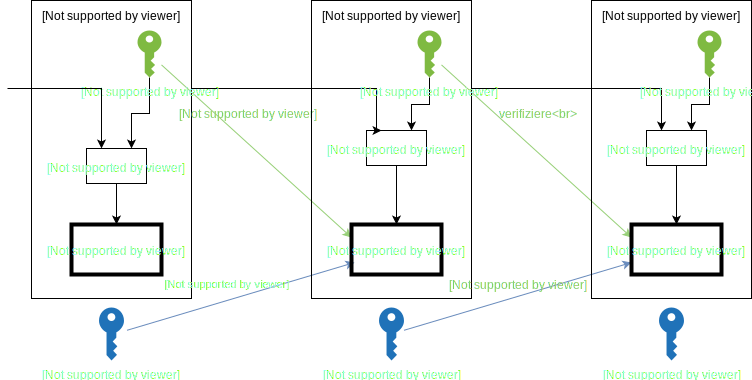
\includegraphics[width=0.9\textwidth]{graphics/transaction.png}
	    	\caption{Kette digitaler Signaturen}
	    	\label{fig:txio}
	    \end{figure}
    
	    Wie in \fref{fig:txio} dargestellt, werden Assets von einem Versender zu einem Empfänger transferiert, in dem der Sender einen Hash der vorigen Transaktion und den öffentlichen Schlüssel des Empfängers mit seinem eigenen privaten Schlüssel digital signiert und diese Hash dann am Ende des Assets anfügt.
	    Transaktionen können zudem mehrere Ein- und Ausgaben haben\cite{Nakamoto2008}.
	    Der Empfänger, sowie alle Teilnehmer des Netzwerkes können den Besitz des Assets über die Kette der digitalen Signaturen zurückverfolgen\cite{Nakamoto2008}.
	    
	    Every signed transaction is broadcasted by a user’s node to its one-hop peers\cite{Christidis2016}
	    
	    The neighboring peers make sure this incoming transaction is valid before relaying it any further; invalid transactions are discarded. Eventually this transaction is spread across the entire network\cite{Christidis2016}
	    
	    The transactions that have been collected and validated by the network using the process above during an agreed-upon time interval, are ordered and packaged into a timestamped candidate block. This is a process called mining. The mining node broadcasts this block back to the network. (The choice of the mining node and the contents of the block depend on the consensus mechanism that the network employs. Refer to Section II-B for more information.)
	    The nodes verify that the suggested block (a) contains valid transactions, and (b) references via hash the correct previous block on their chain. If that is the case, they add the block to their chain, and apply the transactions it contains to update their world view. If that is not the case, the proposed block is discarded. This marks the end of a round.\cite{Christidis2016}
	    
    
    \begin{figure}[H]
        \missingfigure[figheight=4cm]{Bild mit Transaktion}
    \end{figure}
    
    \subsubsection{Smart Contracts}
    
    \subsubsection{Typen}
        Private, Public - Permissioned, Permissionless
        
        Mit einer Blockchain können auch je nach Anwendungsszenario, außer Kryptowährungen, andere (digital repräsentierte) Waren oder Assets wie Güter im Supply Chain Management\cite{Underwood2016}, Identitäten zur Zugangskontrolle\cite{Kshetri2017} oder Proof of Ownership digitaler Rechte\cite{Wuest2017} gespeichert und gehandelt werden. 
        Unterschiedliche Anwendungen haben auch verschiedene Anforderungen an die Blockchain selbst. 
        Zur Zeit haben sich unterschiedliche Typen einer Blockchain herauskristallisiert, wo.
        
        
        {\sloppy\url{https://blockchainhub.net/blockchains-and-distributed-ledger-technologies-in-general/}}
        \begin{itemize}[noitemsep]
            \item in private/\-permissioned ist \gls{pow} und \gls{pos} nicht nötig
        \end{itemize}
    
    \subsubsection{Sicherheit}
    \label{sec:sota_blockchain_security}
        Das System ist so lange sicher, wie ,,ehrliche'` Knoten gemeinsam mehr Rechenleistung als eventuell zusammenarbeitende Angreifer haben\cite{Nakamoto2008}
        Byzantine Fault Tolerance
        Consensus Algorithms
        \begin{itemize}
            \item Users interact with the blockchain via a pair of private/public keys [13]. They use their private key to sign their own transactions, and they are addressable on the network via their public key.2 The use of asymmetric cryptography brings authentication, integrity, and nonrepudiation into the network\cite{Christidis2016}
        \end{itemize}
    
    \subsubsection{Identity Management}
    \label{sec:sota_blockchain_identitymgmnt}

    \subsection{Internet of Things}
\label{sec:sota_iot}
\subsubsection{Sicherheit}
\label{sec:sota_iot_security}
\subsubsection{Protokolle (BLE, Z-WAVE)}
    \cite{Gomez2012}
    In \cite{Rose2016}
    \begin{itemize}
        \item nur kleine Datenmengen können ausgetauscht werden (20Bytes)\cite{Rose2016}
        \item geriner Energieverbrauch
        \item funktioniert wie Bluetooth Classic auf 2,4Ghz
        \item kurze Reichweite (<100m)
        \item verschiedene Hosts mit jeweils verschiedenen Profilen, geht vom Controller aus
    \end{itemize}
    
    \paragraph{Profile}\cite{Rose2016}
        \begin{itemize}
            \item General Attribute Profile (Client schickt Anfrage an GATT Server, Server speichert Attribute)
        \end{itemize}

\label{sec:sota_iot_protocols}
\subsubsection{Smart Home}
\label{sec:sota_iot_smart_home}
    \subsection{Smart Locks}
\label{sec:sota_smart_locks}
	Da sich Architektur und Funktionsmechanismen in manchen Punkten je nach Hersteller unterscheiden, gelten die im Folgenden dargelegten technischen Erklärungen, soweit nicht explizit erwähnt, für das Smart Lock von der Firma August. 
    \medskip\\
    \noindent Smart Locks sind ,,elekromechanische Türschlösser``, die sich dadurch auszeichnen, dass sie für einen Nutzer mit einer Smartphone-App steuerbar sind und mittels eines kabellosen Standards wie Bluetooth (siehe \fref{sec:sota_iot_protocols}) für kurze Distanzen kommunizieren.
	Als ,,Smart Lock`` werden keine Schlösser bezeichnet, bei denen ein physisches Schloss
	\footnote{beispielweise ein Stiftschloss, welches mit einem herkömmlichen Schlüssel geöffnet werden kann} 
	mit einem Ziffernblock ersetzt wurde oder sich nicht mit anderen Geräten innerhalb des \gls{iot} in irgendeiner Weise verbinden.\cite{Ho2016}
	
	\subsubsection{Typische Architekturen und Gemeinsamkeiten}
	    In den den doch sehr unterschiedlichen Produkten, die momentan auf dem freien Markt verfügbar sind oder bisher verfügbar waren, lassen sich trotz alledem einige Gemeinsamkeiten erkennen\cite{Ye2017,Fuller2017}. 
    	\noindent Generell besteht ein Smart Lock-System aus folgenden Bestandteilen (vgl. \fref{fig:sl_arch}):
    	\begin{enumerate}[noitemsep]
    		\item einem elektrischen Schloss oder einer elektronischen Erweiterung eines vorhandenen Schlosses
    		\item mindestens einem Nutzer, welcher durch sein Endgerät, meist ein Smartphone, identifiziert wird
    		\item einem herstellereigenen Server
    		\item einem Webinterface
    		\item optional einem Zubehörgerät, welches erlaubt dem Schloss mit dem Internet zu kommunizieren
    	\end{enumerate}
    
    	\begin{figure}[H]
    		\centering
    		\includegraphics[width=0.9\textwidth]{graphics/august_2.jpg}
    		\caption{Bestandteile eines August Smart Lock Pro\cite{August}}
    		\label{fig:august1}
    	\end{figure}
    
	    \noindent Das Schloss selbst ist an der Außen- und/oder Innenseite einer Tür angebracht (vgl. \fref{fig:august1}) und erweitert ein vorhandenes Schloss elektronisch oder ist selbst in Form eines Vorhängeschlosses\cite{Ho2016}. 
		Zum System gehört in den meisten Fällen eine mobile Applikation für ein Smartphone zum Öffnen und Schließen des Schlosses, sowie zur Administration\cite{Fuller2017}. 
        Eher seltener beinhaltet das Produkt auch eine Weboberfläche, welche ebenfalls für administrative Aufgaben genutzt werden kann\cite{Ho2016}. 
		Es existiert ein herstellereigener (Remote-)Server, auf dem sich eine authoritative Liste aller Nutzer, sowie deren Rechte befindet. 
        Diese bildet die Grundlage zur Realisierung der Zugriffskontrolle.\cite{Fuller2017} 
        Das Öffnen und Schließen erfolgt primär elektronisch mittels eines Buttons per App.
        Alternativ lässt sich das Schloss entweder mit einem sogenannten ,,Keyfob`` 
        \footnote{einem Schlüsselanhänger, auf dem sich ein digitaler Schlüssel befindet} 
        oder einem physischen Schüssel öffnen\cite{Ho2016}. 
        Einige Modelle bieten auch eine Funktion, die die Tür automatisch öffnet sobald sich das Smartphone des Nutzers innerhalb eines bestimmten Radius befindet. 
        Sobald folgende Bedingungen gegeben sind, öffenet sich das Schloss automatisch:
        \begin{itemize}[noitemsep]
        	\item automatisches Öffnen wurde vom Nutzer aktiviert
        	\item der Nutzer hat einen Ort bzw. für Geofencing festgelegt \footnote{Geofencing erklären}\todo[color=cyan]{Geofencing erklären}
        	\item der Nutzer befindet sich in Reichweite, um über sein Smartphone mit dem Schloss kommunizieren zu können
        	\item der Nutzer ist berechtigt das Schloss zu öffnen
        \end{itemize}
    	Verlässt der Nutzer den Radius des Geofencings wieder, wird das Schloss automatisch verriegelt.
		Ein optionales Zubehörgerät fungiert als Relay
		\footnote{leitet Nachrichten von mehreren Entitäten in einem Netzwerk (unverändert) weiter}
		, welches sich per \gls{ble} mit dem Schloss verbindet und über das W-LAN Heimnetzwerk des Nutzers mit dem Internet verbindet.
		
    \subsubsection{Typische Funktionen}
		Um das Schloss zu kontrollieren installiert der Nutzer initial eine herstellerspezifische App auf seinem Smartphone und erstellt ein Nutzerkonto auf dem Server des Herstellers. 
		Danach pairt der Nutzer via \gls{ble} sein Gerät mit dem Schloss.\cite{Ho2016} 
		Die Identifikation der verschiedenen Nutzer für administrative Zwecke erfolgt entweder mittels E-Mailadresse oder Telefonnummer. 
		Aus technischer Sicht werden Nutzer anhand eines einzigartiger Schlüssel identifiziert, die der Besitzer des Schlosses nicht kennt.\cite{Fuller2017}\todo[color=orange]{nachlesen} 
		Die Smart Locks enthalten eine eingebaute Funktion, um Zugriffe zu protokollieren. 
		Dazu gehören Aktionen wie \cite{Fuller2017}:
		\begin{itemize}[noitemsep]
			\item von welchem Nutzer eine Funktion genutzt wurde, 
			\item der Zeitpunkt, an dem das Schloss elektronisch geöffnet oder geschlossen wurde,
			\item der Zeitpunkt, an dem das Schloss manuell geöffnet oder geschlossen wurde
			\item wann, wem und von wem Zugriff gewährt oder entzogen wurde
		\end{itemize}
		Die Logs werden asynchron mit der Smartphone App aktualisiert, sobald sich das Gerät des Nutzers in Reichweite des \gls{ble} befindet\citeauthor{Ho2016}.
	
	\subsubsection{Kommunikation}
		\begin{figure}[H]
			\centering
			\includegraphics[width=\textwidth]{graphics/sl_arch.png}
			\caption{Beispiel eines Smart Lock-Systems}
			\label{fig:sl_arch}
		\end{figure}

        nach \citeauthor{Ho2016}:
        In \fref{fig:sl_arch} abgebildet: Smart Lock hat keine Internetverbindung. 
        Endgerät des Nutzers übernimmt die Funktion eines Proxy/Gateway, welches Informationen zwischen dem Smart Lock und den Servern des Herstellers überträgt. 
        Dies setzt voraus, dass sich das Endgerät in Kommunikationsreichweite für das jeweilige Protokoll (bspw. \gls{ble}) befindet. 
        Direkte Internetverbindung des Smart Locks zur Kommunikation mit dem Server des Herstellers mittels eingebautem Wifi-Modem, welches sich mit dem Netzwerk des Nutzers verbindet. 
        Die Informationen über Rechtevergaben und Gerätezustand etc. werden hier allerdings über das Internet und nicht über lokale Kommunikation (wie \gls{ble}) übertragen. 
        \gls{ble} zwischen Smartphone und Smart Lock wird verwendet für: 
        \begin{itemize}
            \item Athentifizierung des Smartphones des Nutzers 
            \item Nachrichten mit Informationen über gewährten und entzogenen Nutzerrechten
            \item die Smartphone-App bzw. die Logs über Aktivitäten (lock/unlock) informieren
        \end{itemize}

    \subsubsection{Sichereit}
        \paragraph{Rollen und Rechteverteilungen:}
        Relevant: \cite{Ye2017}\cite{Ho2016}
		\subparagraph{Rollen:} Owner(Grant, Revoke, Lock/Unlock, Admin Features wie Zugriffshistorie Lediglich der Nutzer mit der Rolle des Owners kann diese Protokolle einsehen. ), Resident(Lock/Unlock), wiederkehrender Gast (nur Lock/Unlock zu bestimmten Zeitfenstern), temporärer Gast(Lock/Unlock für eine bestimmte Zeit wie 24 Stunden) 
		Die Rolle des Owners wird jenem Gerät vergeben, das sich nach Installation des Smart Locks als erstes mittels \gls{ble} (oder bei einigen Modellen über W-LAN) verbindet. 
   		Die Owner-Rolle kann auf diesem Wege nur einmal vergeben werden. 
   		Bei Wechsel des Besitzers muss das Smart Lock zurückgesetzt werden. 
   		Rollen wieder zu entfernen und somit anderen Nutzers wieder die Rechte zu entziehen, muss Owner sein. 
   		Um die Rechte eines Owners bei einem verlorenen oder gestohlenen zu entziehen, wird entweder eine "Lost Phone"-Funktion angeboten oder ein anderer Nutzer mit der Rolle des Owners entzieht dem nicht mehr vorhandenen Gerät die Rolle. 
   		Der Owner kann das Schloss auch ohne Internetverbindung öffnen/schließen. 
   		Gäste hingegen müssen sich vor der Kommunikation mit dem Schloss gegenüber der dem Server des Herstellers autorisieren lassen. 
		\subparagraph{Rechte:} Lock/Unlock, Lock Activity, Guest List, User Invitation (new Users), User Level Control (update User Role), User Permission Control (e.g. set time slots for guests, revoke permissions from users), Schloss kalibrieren und zurücksetzen\cite{Fuller2017}, Activiy Protokoll ansehen\cite{Fuller2017}, Autolocking/-unlocking akivieren/deaktivieren, eigenen Account löschen
		
		\paragraph{Secret Keys}
		über Secret Keys\cite{Fuller2017}
		\begin{itemize}
		    \item jede Bluetooth-Verbindungssession bekommmt einen eigenen einzigartigen Session-Key (weiter SK genannt), welcher für Owner wie folgt entsteht:
		    \missingfigure{Wie der Session Key für Owner entsteht}
		        \begin{enumerate}
		            \item Das Smartphone sendet zufällige 64 Bit an das Schloss, welche mit dem offline Keys des Smartphones verschlüsselt werden, an das Schloss
		            \item Das Schloss sendet 64 zufällige Bits, die mit dem offline Key des Smartphones verschlüsselt sind, an das Smartphone zurück
		            \item Das Schloss und das Smartphone entschlüsseln die jeweils erhaltene Nachricht und konkatinieren beide Nachrichten zu einer neuen 128-Bit langen Folge, die im weiteren Verlauf als AES-Key zur Verschlüsselung der Session genutzt wird.
		        \end{enumerate}
		        Gäste, welche keinen "offline Key" zugewiesen bekommen, kommunizieren mit dem Webserver:
		        \missingfigure{Wie der Session Key für Gäste entsteht}
		        \begin{enumerate}
		            \item Das Smartphone des Gasts sendet 64 zufällige Bits als Klartext an den Server
		            \item Der Server verschlüsselt diese 64 Bits mit dem Firmware Key und sendet die verschlüsselten Bits als Nachricht an den Gast zurück
		            \item Der Gast leitet den Ciphertext, welcher von dem Server empfangen wurde, an das Schloss weiter.
		            \item Das Schloss sendet 64 Bits mit XY  verschlüsselt an den Gast, welcher diesen Ciphertext an den Server weiterleitet.
		            \item Der Server entschlüsselt die Nachricht und sendet sie als Klartext per SSL an den Gast.
		            \item Das Schloss und der Gast konkatenieren beide 64-Bit langen Folgen zu einem 128-Bit Schlüssel, welcher als Session Key verwendet wird.
		        \end{enumerate}
		    \item SK wird genutzt, um Nachrichten zwischen dem Schloss und dem Smartphone des Nutzers mit AES zu ver- und entschlüsseln
		    \item Voraussetzung: für das Protokoll, welches den Session Key erstellt müssen bereits im Voraus das Schloss und entweder die Webserver des Herstellers oder das Smartphone des Nutzers einen Secret Key teilen.
		    \item in August können insgesamt 256 Schlüssel (von 0-255 nummeriert) gespeichert werden, wobei Nummer 0 besondere Privilegien hat und als "firmware key" angesehen wird (\textrightarrow Hardcoded und somit anfällig, sollte in falsche Hände geraten).
		        Die Webserver des Herstellers, Nutzer mit der Rolle OWNER und das Schloss selbst kennen den Schlüssel.
		        anderen Keys sind "offline Keys", die zur Initialisierung einer Bluetooth-Session verwendet werden, sollte der Nutzer nicht mit dem Internet verbunden sein
		\end{itemize}
		
		

    \subsection{Sicherheitsanalysen im Internet of Things}
\label{sec:sota_sa}
	
	\begin{itemize}
		\item Sicherheitskonzepte erklären, Sicherheitsziele (CIA, Auth, Non-rep, etc.)
		\item Erwähnung von OWASP-Projekt und Guidelines
		\item \gls{cvss} Bewertungsschema erklären
		\item Threat Model
		\item Securityl Goals
	\end{itemize}
	Kurze Einfühung, dann gleich Überleitung zum CVSS.
	
	\cite{CVSSspec}
	Confidentiality refers to limiting information access and disclosure to only authorized users, as well as preventing access by, or disclosure to, unauthorized ones.
	
	Integrity refers to the trustworthiness and veracity of information.
	
	Since availability refers to the accessibility of information resources, attacks that consume network bandwidth, processor cycles, or disk space all impact the availability of an impacted component.
	
\subsubsection{Common Vulnerability Scoring System (CVSS)}
\label{sec:sota_sa_cvss}
    \todo[color=cyan]{System kurz erlöären}
    \noindent Der Base Score besteht aus zwei Subscores, Exploitability Score und Impact Score, welche wie folgt in Listing \ref{eq:cvss_basescore} verrechnet werden:
    \begin{lstlisting}[caption={Berechnung des BaseScore \cite{CVSSspec}},label=eq:cvss_basescore,captionpos=b,mathescape=true]
if (ImpactSubScore <= 0)
    BaseScore = 0
else
if(Scope == Unchanged)
    BaseScore = RoundUp(Minimum [(Impact + Exploitability), 10])
if(Scope == Changed)
    BaseScore = RoundUp(
      Minimum [1.08 $\mathsf{\times}$ (Impact + Exploitability), 10])
    \end{lstlisting}
    
    \noindent Ziel des Base Scores ist es wesentliche Charakteristiken, die in verschiedenen Umgebungenen und Zeitpunkten konstant sind, einer Schwachstelle zu repräsentieren. 
    Der Score liegt zwischen dem Wert 0.0 und 10.0, wobei 0 das kleinste Risiko repräsentiert und 10 das Größte\cite{CVSSspec}. 
    Die \fref{tab:cvss_severity} zeigt die Zuordnung der verschiedenen Scores zu Risikograden. 
    \begin{table}[H]
        \centering
        \begin{tabular}{|m{0.2\textwidth}|m{0.2\textwidth}|}
        \hline
        \textbf{Rating}   & \textbf{\gls{cvss} Score}   \\ \hline
        None              & 0.0                         \\ \hline
        Low               & 0.1 - 3.9                   \\ \hline
        Medium            & 4.0 - 6.9                   \\ \hline
        High              & 7.0 - 8.9                   \\ \hline
        Critical          & 9.0 - 10.0                  \\ \hline
        \end{tabular}
        \caption{Skala des Ausmaßes\cite{CVSSspec}}
        \label{tab:cvss_severity}
    \end{table}
    \noindent Der Exploitability Score wird aus den Exploitablility Metrics berechnet(vgl. Listing \ref{eq:cvss_explscore}) und modelliert die Charakteristiken der anfälligen Komponente. 
    \smallskip\\
    \begin{lstlisting}[caption={Berechnung des Exploitability Score \cite{CVSSspec}},label=eq:cvss_explscore,captionpos=b,mathescape=true]
Exploitability = 8.22 $\mathsf{\times}$ AttackVector $\mathsf{\times}$ AttackComplexity 
  $\mathsf{\times}$ PrivilegeRequired $\mathsf{\times}$ UserInteraction
    \end{lstlisting}
    \noindent Folgende Variablen werden dabei verrechnet:
    \begin{description}[itemsep=0.7em,align=left,labelindent=0pt,leftmargin=0pt]
        \item [Attack Vector:] Beschreibt den Kontext, in der Ausnutzung der Schwachstelle möglich ist.
            Der Wert, der in den Exploitability Score einfließt ist größert, je entfernter (im technischen Sinne) ein Angreifer sein kann, um einen Angriff zu starten.
            \begin{description}[noitemsep,align=left,labelindent=0.7cm,leftmargin=0.7cm]
                \item [Network:] Schwachstelle ist über Netzerkzugriff ausnutzbar, auch, wenn der Zugriff ein oder mehrere Hops via Layer 3
                \footnote{nach dem OSI-Modell}
                entfernt ist. 
                \item [Adjacent:] Schwachstelle ist über Netzerkzugriff ausnutzbar, aber der Angriff ist auf das selbse physische oder logische Netzwerk eingeschränkt und kann nicht über eine Layer 3 Grenze (bspw. einem Router) ausgeführt werden.
                \item [Local:] Ein lokaler Zugriff ist nötig, um die Schwachstelle ausnutzen zu können und die Komponente ist nicht an den Netzwerkstack gebunden.
                Der Angriff funktioniert über lesende/schreibende/ausführende Zugriffe und kann voraussetzen, dass der Angreifer entweder in das System eingeloggt ist und/oder eine Nutzerinteraktion tätigt, bei der eine bösartige Datei ausgefürt wird.
                \item [Physical:] Der Angreifer muss in der Lage sein die anfällige Komponente über eine bestimmte Zeit physisch zu bedienen oder zu manipulieren.
            \end{description}
        \item [Attack Complexity:] Beschreibt die Bedingungen außerhalb der Kontrolle des Angreifers, die herrschen müssen, um die Schwachstelle auszunutzen (bspw. bestimmte Systemkonfiguration).
            \begin{description}[noitemsep,align=left,labelindent=0.7cm,leftmargin=0.7cm]
                \item [Low:] Spezielle Zugriffsbedingungen oder ähnliches existieren nicht.
                Ein Angreifer kann wiederkehrenden Erfolg gegen die Komponente erzielen.
                \item [High:] Ein erfolgreicher Angriff hängt von Zuständen außerhalb des Einflusses des Angreifers ab und kann voraussetzen, dass der Angreifer im Voraus einiges an Aufwand investieren muss, um diese Zuständer herzustellen.
            \end{description}
        \item [Privileges Required:] Beschreibt das Level an Privilegien, die ein Angreifer besitzen muss, um eine Schwachstelle ausnutzen können.
            \begin{description}[noitemsep,align=left,labelindent=0.7cm,leftmargin=0.7cm]
                \item [None:] Der Angreifer ist vor dem Angriff nicht autorisiert und benötigt daher keinen Zugriff auf Einstellungen oder Dateien, um den Angriff ausführen zu können.
                \item [Low:] Der Angreifer ist mit grundlegenden Nutzerrechten autorisisiert.
                \item [High:] Der Angreifer ist mit erweiterten oder administrativen Rechten autorisiert und kann komponentenweite Einstellungen und Dateien ändern.
            \end{description}
        \item [User Interaction:] Beschreibt die Voraussetzung, ob ein Angreifer einen erfolgreichen Angriff ohne weitere Beteiligung von anderen Nutzern ausführen kann oder ob ein Nutzer in irgendeiner Weise mitwirken muss.
            \begin{description}[noitemsep,align=left,labelindent=0.7cm,leftmargin=0.7cm]
                \item [None:] Ein Angriff kann ohne Interaktion eines anderen Nutzers erfolgreich sein.
                \item [Required:] Erfolgreiches Ausnutzen einer Schwachstelle ist nur möglich, wenn ein anderer Nutzer eine oder mehrere bestimmte Aktionen ausführt.
            \end{description}
    \end{description}
    
    \noindent Der Impact Score wird aus den Impact Metrics berechnet (vgl. Listing \ref{eq:cvss_impscore} und beschreiben die Eigenschaften des betroffenen Komponenten. 
    Sollte ein erfolgreich ausgeführter Angriff auch andere Komponenten beeinflussen, so wird die Komponente mit dem worst-case, also der höchsten Einstufung gewertet.
    \smallskip\\
    \begin{lstlisting}[caption={Berechnung des Impact Score \cite{CVSSspec}},label=eq:cvss_impscore,captionpos=b,mathescape=true]
$\mathsf{ISC_{Base}}$ = 1 - [(1 - $\mathsf{Impact_{Conf}}$) $\mathsf{\times}$ (1 - $\mathsf{Impact_{Integ}}$) $\mathsf{\times}$ (1-$\mathsf{Impact_{Avail}}$)]
if (Scope == Unchanged)
    Impact = 6.42 $\mathsf{\times}$ $\mathsf{ISC_{Base}}$
if (Scope == Changed)
    Impact = 7.52 $\mathsf{\times}$ [$\mathsf{ISC_{Base}}$ - 0.029] - 3.25 $\mathsf{\times}$ [$\mathsf{ISC_{Base}}$ - 0.02]$\mathsf{^{15}}$
    \end{lstlisting}
    \begin{description}[itemsep=0.7em,align=left,labelindent=0pt,leftmargin=0pt]
        \item [Confidentiality:] Ausmaß auf die Vertraulichkeit der Informationsressourcen, die von einer Softwarekomponente verwaltet werden, welche durch das Ausnutzen einer Schwachstelle komprommittiert wurde.
            \begin{description}[noitemsep,align=left,labelindent=0.7cm,leftmargin=0.7cm]
                \item [None:] Kein Verlust der Vertraulichkeit.
                \item [Low:] Der Angreifer erlangt eingeschränkt Zugriff auf Informationen, hat aber keine Kontrolle darüber, welcher Informationen er erlangt.
                    Oder: Die Preisgabe der Informationen verursacht keinen direkten, schweren Verlust bei der betroffenen Konponente.
                \item [High:] Die Vertraulichkeit ist nicht mehr gegeben.
            \end{description}
        \item [Integrity:] Ausmaß auf die Integrität der Informationsressourcen, die von einer Softwarekomponente verwaltet werden, welche durch das Ausnutzen einer Schwachstelle komprommittiert wurde.
            \begin{description}[noitemsep,align=left,labelindent=0.7cm,leftmargin=0.7cm]
                \item [None:] Kein Verlust der Integrität.
                \item [Low:] Änderung von Daten durch einen Angreifer ist möglich, aber der Angreifer selbst hat keine Kontrolle über die Konsequenz seiner Modifikation oder das Maß der Modifikation ist eingeschränkt.
                \item [High:] Verlust jeglicher Integrität.
                    Der Angreifer kann alle Daten, die durch die Komponente geschützt oder kontrolliert werden modifizieren.
            \end{description}
        \item [Availability:] Ausmaß auf die Verfügbarkeit der Informationsressourcen, die von einer Softwarekomponente verwaltet werden, welche durch das Ausnutzen einer Schwachstelle komprommittiert wurde.
            Damit ist der Verlust der Verfügbarkeit der betroffenen Komponente (wie ein Webservice, eine Datenbank, etc.) selbst gemeint.
            \begin{description}[noitemsep,align=left,labelindent=0.7cm,leftmargin=0.7cm]
                \item [None:] Kein Verlust der Verfügbarkeit
                \item [Low:] Reduzierte Leistung oder Unterbrechungen in der Verfügbarkeit der Ressource.
                \item [High:] Kompletter Verlust der Verfügbarkeit, was dazu führt, dass ein Angreifer den Zugriff auf Ressourcen innerhalb der betroffenen Komponente verhindern kann.
            \end{description}
    \end{description}
    
    \begin{description}[itemsep=0.7em,align=left,labelindent=0pt,leftmargin=0pt]
        \item [Scope:] Beeinflusst ein erfolgreicher Angriff mindestens eine andere Komponente außer die Anfällige?
            \begin{description}[noitemsep,align=left,labelindent=0.7cm,leftmargin=0.7cm]
                \item [Unchanged:] Eine ausgenutzte Schwachstelle beeinflusst nur Ressourcen, die von der gleichen Authorität verwaltet werden - anfällige und die betroffene Komponenten sind also identisch.
                \item [Changed:] Eine ausgenutzte Schwachstelle kann Ressourcen außerhalb der Komponente beeinflussen - anfällige und die betroffene Komponenten sind also nicht identisch.
            \end{description}
    \end{description}
    
    \noindent Es existieren Erweiterungen des Base Scores, der Temporal Score und Environmental Score. 
    Diese beiden Werte werden in dieser Arbeit nicht verwendet. 
    Für die genauen Werte, die für die Berechnungen verwendet werden, wird auf \cite{CVSSspec} verwiesen.\todo[color=cyan]{Anhang?}
    
    \newpage
    \section{Analyse}
\label{sec:analysis}
	Um spezielle Anforderungen für den Prototypen festlegen zu können, werden zunächst bekannte Sicherheitslücken von bestehenden Produkten analysiert. 
	Als Schwachstellen und Sicherheitslücken werde jene aufgenommen, die zumindest in einem Produkt entdeckt und vor dem Zeitpunkt der Erstellung dieser Arbeit veröffentlicht wurden.
	
	Zunächst werden einige bekannte Schwachstellen und/oder Sicherheitslücken kurz vorgestellt.
	Um die Basis für eine Vergleichbarkeit zwischen vorhandenen Produkten und dem in dieser Arbeit entwickelten Prototypen zu gewährleisten, werden gefundene Schwachstellen und Sicherheitslücken kategorisiert und nach dem \gls{cvss}-Basis Score bewertet.
	Aus diesen Ergebnissen lassen sich einige spezielle Anforderungen an den Prototypen ableiten, die in \fref{sec:analysis_requirements} erläutert werden.
	\todo[color=green]{KL}

    \subsection{Bekannte Schwachstellen und Angriffe}
\label{sec:analysis_vulns}
    Es werden nach Literaturrecherche hier einige Schwachstellen und Angreiffe vorgestellt. 
    Die Kategorisierung nach den \gls{owasp} Top Ten \gls{iot} Vulnerabilities\cite{Miessler2015}. 
    Sollte eine Schwachstelle in mehrere Kategorien passen, so wird sie in jene eingeordnet, in der der größte Schaden im Falle eines Angriffs entsteht.\todo[color=yellow]{besser formulieren}
    Für weitere Details zu den im Folgenden beschriebenen Schwachstellen wird auf die jeweiligen Quellen verwiesen.
    \todo[color=orange]{\cite{Tierney2018}\cite{Stykas2018}}

    \subsubsection*{I1: Insecure Web Interface}
       \begin{itemize}[leftmargin=0cm,label={}]
            \item \emph{Insecure API: User Enumeration}\cite{Fuller2017,Lariviere2015}\label{vuln:user_enum}\\
                Produkt: August\\
                Voraussetzungen: \\
                Die in \fref{sec:sota_smart_locks} vorgestellte Kommunikation via Wifi zwischen dem Webserver: 
                Wenn sich ein Nutzer das erste Mal in der App anmeldet, wird eine zufällige ID generiert (installID), welche an den Webserver gesendet wird und für viele API-Aufrufe entweder als Teil des API-Keys oder zusätzlich zu diesem verwendet wird. 
                Die API Endpunkte authentifizieren den Nutzer nicht und erlauben es einem Angreifer einen Gästezugang anzulegen, wenn dieser die \gls{uuid} kennt.
                Diese kann wiederrum durch das Nutzen einer Funktion in der Smartphone-App, welche nach Smart Locks in Reichweite sucht, erlangt werden. 
       \end{itemize} 
       
    \subsubsection*{I2: Insecure Authentification/Authorization}
        \begin{itemize}[leftmargin=0cm,label={}]
            \item \emph{Insufficient Password Protection}\cite{Ye2017}\label{vuln:pwd_prot}\\
    	        Produkt: QuickLock Smart Lock\\ 
                Voraussetzungen: keine\\
                Wird die ,,Passwort vergessen``-Funktion genutzt, so wird dem Nutzer sein verwedetes Passwort zugesendt. 
                Das übertragene Passwort wird allerdings nicht verschlüsselt.
            \item \emph{Insecure API: Privilege Escalation}\cite{Fuller2017,Lariviere2015}\label{vuln:priv_esc}\\
                Produkt: August\\
                Voraussetzungen: \\
                Die in \fref{sec:sota_smart_locks} vorgestellte Kommunikation via Wifi zwischen dem Webserver: 
                Ebenfalls möglich war eine Privilege Escalation, in dem ein String von 'user' auf 'superuser' geändert wurde.
            \item \emph{Insecure Password Policy}\cite{Rose2016,Ye2017,Jmaxxz2015a}\label{vuln:pwd_pol}\\
                Produkt: Quicklock Smart Lock, August Smart Lock\\
                Voraussetzungen: keine\\
                Quicklock: 8-Ziffern PIN (100.000.000 Kombinationen)\\
                August: Verifikation über Rufnummer enthält einen Code mit 6 Ziffern (1.000.000 Kombinationen)\\
                Sollte kein Rate-Limiting im Server vorhanden sein, könnte der Angreifer mit beispielsweise 50 Versuchen pro Sekunde (bei 20ms Netzwerkverzögerung) ide 1.000.000 Kombinationen innerhalb von maximal 5-6 Stunden knacken.
            \item \emph{Phishing?}\cite{Ye2017}\label{vuln:phishing}\\
    	        Produkt: August Smart Lock\\ 
                Voraussetzungen: keine\\
                Der Angreifer bringt den Nutzer dazu eine bösartige App zu verwenden, welche der Legitimen sehr ähnlich sieht. 
                Da keine Authentifizierung zwischen Schloss und Nutzer durchgeführt wird, ist dies nur sehr schwer vom Nutzer zu erkennen.
            \item \emph{Replay}\cite{Tierney2018,Rose2016,Ho2016}\label{vuln:replay}\\
                Produkt: Tapplock Smart Lock, Ceomate Bluetooth, Elecycle Smart Padlack, Vians Bluetooth Smart Doorlock, Lagute Sciener Smart Doorlock\\
                Voraussetzungen: \\  
                Vom Nutzer übertragene Befehle zwischen Smartphone und Schloss werden eine Zeit lang aufgezeichnet und zu einem späteren Zeitpunkt wieder abgespielt. 
                Hat sich der Nutzer innerhalb dieser Zeitspanne beispielsweise gegenüber dem Schloss authentifiziert, so kann sich der Angreifer mit dem abgespielten Befehl als der Nutzer authentifizieren.\todo[color=yellow]{doof formuliert}
                Ein Angreifer folgt Alice (außerhalb des Bluetooth- und Geofencingradius, aber in Bluetooth-Reichweite zu Alices Gerät) und überträgt das Signal an einen anderen Angreifer, der vor Alices Haus mit einem bluetoothfähigen Gerät wartet und mittels des übertragenen Signals nun alle Bedingungen erfüllt und das Schloss entriegeln kann.
                Bei Systemen mit Geofencing muss zusätzlich Alices Standort gespooft werden.
            \item \emph{Device Spoofing}\cite{Rose2016}\label{vuln:spoofing}\\
                Produkt: Mesh Motion Bitlock Padlock\\
                \begin{enumerate}[noitemsep]
    	            \item Angreifer gibt sich als Schloss aus, um das Passwort des Nutzers zu stehlen
    	            \item möglich, da ein vorhersehbarer Nonce geschickt wird und die App beim Nutzer im Hintergrund läuft und Befehle ohne Nutzerinteraktion sendet.
    	        \end{enumerate}
	        \item \emph{Missing 2-Factor Authentication}\cite{Jmaxxz2015}\label{vuln:2-factor}\\
                Produkt: August Smart Lock\\
                Voraussetzungen: \\  
                Proof of Posession: E-Mail, Handynummer\\
                Proof of Knowledge: Passwort
                \begin{enumerate}[noitemsep]
                    \item Nutzer benutzt die ,,Passwort vergessen`` Funktion auf einem Smartphone, auf dem der Nutzer bereits mindestens einmal angemeldet war.
                    \item Hersteller sendet Token an die E-Mailadresse des Nutzers.
                    \item Nutzer kann sein Passwort ändern.
                \end{enumerate}
                \begin{enumerate}[noitemsep]
                    \item Nutzer nutzt die ,,Passwort vergessen`` Funktion auf einem Smartphone, auf dem noch kein Nutzer angemeldet war.
                    \item Hersteller sendet Token an E-Mailadresse und Rufnummer des Nutzers.
                        Der Token, der der Rufnummer zugesandt wird muss vor dem Zurücksetzen des Passwortes eigegeben werden.
                    \item Um in dieser Situation zwei Faktoren zur Authentifizierung zu haben, müsste laut \cite{Jmaxxz2015} die Kontrolle über die Rufnummer oder die E-Mailadresse als Proof of Knowledge gelten.
                        Wird eines der beiden Faktoren als Proof of Knowledge defniniert erhält man einen Widerspruch und somit auch keine Authentifizierung über zwei Faktoren, sondern nur über einen Faktor.
                \end{enumerate}
        \end{itemize}
        
    \subsubsection*{I3: Insecure Network Services}
        \begin{itemize}[leftmargin=0cm,label={}]
            \item \emph{Denial of Service via Commands}\cite{Ye2017}\label{vuln:dos_cmd}\\
    	        Produkt: August Smart Lock \\ 
                Voraussetzungen: Angreifer hat Zugriff auf das Smartphone eines Nutzers und auf dem Smartphone selbst Root-Rechte\\
                Winn mehrere Nutzer gleichzeitig versuchen sich mit dem Schloss zu verbinden, wird die App suspendiert, sodass niemand gleichzig Öffnen/\-Schließen-Befehle senden kann. 
    		    Somit kann ein Angreifer kontinuierlich wechseln Öffnen/Schließen-Befehle senden und der legitime Nutzer kann die Smart Lock nicht kontrollieren. 
		    \item \emph{Denial of Service (via manufacturer's server)}\cite{Ye2017}\label{vuln:dos_server}\\
                Produkt: Lockitron\\
                Voraussetzungen: im WLAN Bereich des Nutzers
                direkte Verbindung des Schlosses mit den Servern des Herstellers \textrightarrow legitime Nutzer könnten ausgeschlossen werden, wenn dessen Server nicht erreichbar sind
            \item \emph{Denial of Service via Bluetooth}\cite{Ye2017}\label{vuln:dos_ble}\\
    	        Produkt: alle\\ 
                Voraussetzungen: keine\\
                Der Angreifer nutzt einen Bluetooth-Jammer, um die Kommunikation zwischen Smartphone und Schloss zu unterbinden. 
                Aufgrund der in \fref{fig:gateway_arch} vorgestellten Architektur sind somit keine Dienste mehr verfügbar. 
            \item \emph{Access Log Evasion}\cite{Ho2016}\label{vuln:access_log_evasion}\\
                Produkt: August, Danalock, Kevo, Okidokeys, Lockitron\\
                Voraussetzungen: \\
                ist möglich, da, wie in dem oben beschriebenen Szenario davon ausgegangen wird, dass alle Geräte alle Aktionen an den remote Server senden.
                Szenario mit Danalock: Alice, Bob und Mallory haben einen legitimen Zugang.
                Bob ist Owner und kann die Access Logs einsehen.
                Mallory blockiert alle Pakete, die von der App an den remote Server gesendet werden während er mit dem Schloss via ÖFFNEN/\-SCHLIEßEN- Befehl interagiert.
                Somit werden seine Aktionen nicht mitgeschrieben, da das Schloss selbst diese Aktionen von Schloss selbst nicht zwischengespeichert und über einen anderen Client an den remote Server gesendet werden.
                Da diese Informationen auch nachdem Alice mit dem Schloss interagiert nicht über ihr Gerät an den Server weitergeleitet werden, kann Bob als Owner nicht sehen, dass Mallory das Schloss geöffenet oder geschlossen hat.
        \end{itemize}
        
    \subsubsection*{I4: Lack of Transport Encryption/Integrity Verification}
        \begin{itemize}[leftmargin=0cm,label={}]
            \item \emph{Insecure Password Transmission}\cite{Rose2016}\label{vuln:pwd_trns}\\
                Produkt: Quicklock, iBluLock, Pantraco Phantomlock\\
                Voraussetzungen: \\ 
                Plain Text Password: z.B. einfach Opcode (Herstellserspezifisch), aktuelles Passwort, neues Passwort konkatiniert und gesendet. 
    	        Wird dies gesendet, dann wird der Owner mit einem neuen Passwort ausgesperrt und ein hard Reset ist nötig. 
    	        Jedoch ist diser Angriff nur möglich, wenn das Schloss in dem Moment, in dem die Nachricht gesendet wird, entriegelt ist.
            \item \emph{Insecure Bluetooth-Pairing - Session Key}\cite{Fuller2017}\label{vuln:ble_sk}\\
                Produkt: August\\
                Voraussetzungen: \\
                der Session Key wird als Klartext vom Server an den Gast geschickt, sodass ein Mithörer an diesen gelangen könnte.
    	        Er wird jedoch unverzüglich für die Kommunikation zwischen Schloss und Gast genutzt und direkt nach Nutzung wieder verworfen, sodass das Kennen des Session Keys für einen Angreifer laut \citeauthor{Fuller2017} eher unwahrscheinlich einen Nutzen hervorbringt.
	        \item \emph{Revocation Evasion}\cite{Fuller2017,Ho2016}\label{vuln:revocation_evasion}\\
                Produkt: August, Danalock, Kevo, Okidokeys, Lockitron\\
                Voraussetzungen: \\
                Indem ein Angreifer, dessen Rechte entzogen werden soll jegliche Kommunikation zwischen Alice und dem remote Server des Herstellers verhindert.
                Dies kann beispielsweise am einfachsten mittels des Flugmodus erreicht werden.
                Gleichzeitig entgeht der Angreifer auch dem Access Logging.
                Szenario mit Danalock: Alice möchte Mallory, einem Nutzer mit temprärem Zugang die Rechte entziehen. 
                Dazu nutzt sie die App, welche diese Information an den Server des Herstellers sendet und ihr sofort bestätigt, dass sie Rechte von Mallory nun entzogen wurden. 
                Dieser sendet eine Benachrichtigung darüber an Mallorys Gerät. 
                Befindet sich Mallorys Gerät zu diesem Zeitpunkt im Flugmodus, erreicht diese Benachrichtigung ihr Ziel nicht und das Schloss selbst bleibt unwissend über dieses Ereignis. 
                Selbst, wenn ein legitimes Gerät mit dem Schloss interagiert, wird die Benachrichtung über Mallorys Entzug der Recht nicht vom Server über jenes übertragen.
                Somit behält Mallory Zugang für das Schloss. 
                Oder: in Angreifer mit einem in der Zukunft auf Zeit limitierten Gastzugang ändert die Zeiteinstellung auf seinem Gerät, um zu einem anderen Zeitpunkt Zugriff zu erhalten
            \item \emph{Decompiling APKs}\cite{Rose2016}\label{vuln:decompile}\\
                Produkt: Poly-Control Danalock Doorlock\\
                Voraussetzungen: \\  
                \begin{enumerate}[noitemsep]
    	            \item APKs vom Android-Gerät holen
    	            \item .dex zu .jar konvertieren
    	            \item .jar dekompilieren
    	            \item zeigt Verschlüsselungsmethode und hardcoded Secret (Kerckoff's Prinzip)
    	            \item XOR(passwort, secret) \textrightarrow es ist also einfach an das Passwort zu kommen \textrightarrow Entschlüsseln der Kommunikation ist möglich
    	        \end{enumerate}
        \end{itemize}
        
    \subsubsection*{I5: Privacy Concerns}
        \begin{itemize}[leftmargin=0cm,label={}]
            \item \emph{Extracted User Data}\cite{Lariviere2015,Ye2017}\label{vuln:user_data}\\
                Produkt: August Smart Lock\\ 
                Voraussetzungen: Angreifer hat Zugriff auf das Smartphone eines Nutzers\\
                Jegliche gesammelten persönlichen Informationen, die für die Anmeldung der App benötigt werden, werden auf dem Smartphone des Nutzers mit \gls{aes} verschlüsselt abgelegt. 
                Der verwendete Modus der \gls{aes}-Versclüsselung ist \gls{ecb}, wobei der verwendete Schlüssel hardcoded und als Klartext in der Smartphone-App abgelegt wird. 
    		    Ein Angreifer, der Zugriff auf das Smartphone von Alice hat, kann also u.a. UserId, Namen, Rufnummer und Profilbild von Alice auslesen.
        \end{itemize}
        
    \subsubsection*{I6: Insecure Cloud Interface}
        \begin{itemize}[leftmargin=0cm,label={}]
            \item 
        \end{itemize}
        
    \subsubsection*{I7: Insecure Mobile Interface}
        \begin{itemize}[leftmargin=0cm,label={}]
            \item \emph{Stolen User Settings}\cite{Ye2017}\label{vuln:user_settings}\\
                Produkt: August Smart Lock\\ 
                Voraussetzungen: Angreifer hat Zugriff auf das Smartphone eines Nutzers und auf dem Smartphone selbst Root-Rechte\\
                Mallory kopiert die Einstellungen der App, welche als eine bestimmte Datei auf dem Smartphone von Alice gespeichert werden.
    		    Mallory legt sich einen neuen Account an und nutzt dafür die kopierten Einstellungen. \textrightarrow Mandatory Access Control 
    		    Nun wird der Angreifer als legitimer Nutzer angesehen.
    		    Dies beinhaltet die Verwendung von jeglichen administrativen Funktionen wie das Ändern der Gästeliste. 
		    \item \emph{Insecure Bluetooth-Pairing}\cite{Tierney2018,Rose2016,Ye2017,Fuller2017}\label{vuln:ble_pairing}\\
                Produkt: August Smart Lock, Tapplock Smart Lock\\
                Voraussetzungen: keine\\
                August: Das Bluetooth-Pairing zwischen Schloss und Alices Smartphone wird über die Passkey-Methode vollzogen. 
                Der verwendete Handshake-Key ist statisch und ist in den Dateien, welche die Einstellungen der App enthalten, als Klartext auf Alices Smartphone zu finden. 
                Zudem wird keine Authentifizierung zwischen beiden Entitäten durchgeführt und in den Zugriffsprotokollen ist nicht erkennbar, dass ein Angreifer mit dem Schloss interagiert hat. 
                Kann exploited werden (mit Proof of concept auf Github)\\
                Tapplock: Der Key für das Bluetooth-Pairing ist ein MD5-Hash, welcher aus der Konkatenierung der \gls{ble}-Mac-Adresse und der Seriennummer berechnet wird.
        \end{itemize}
        
    \subsubsection*{I8: Insufficient Security Configurability}
        Nicht mittels \gls{cvss} bewertbar
        
    \subsubsection*{I9:Insecure Software/Firmware}
        \begin{itemize}[leftmargin=0cm,label={}]
            \item \emph{Fuzzing}\cite{Rose2016}\label{vuln:fuzzing}\\
                Produkt: Okidokey Smart Doorlock\\
                Voraussetzungen: \\  
                Indem man einige Bytes eines gültigen Befehls ändert und versucht das Schloss in einen Fehlerzustand zu bringen. 
    	        Okidokey:
    	        \begin{enumerate}[noitemsep]
    	            \item über Sniffing an einen gültigen Befehl kommen, bei dem ein scheinbar einzigartiger Schlüssel gesendet wird
    	            \item indem man das dritte Byte zu 0x00 ändert, bringt man das Schloss in einen Fehlerzustand, in welchem sich das Schloss automatisch entriegelt\\
    	            \lstinline{9348(Opcode?)|llub6cad7299ec1481791303d7c90d549352398(Key)}
    	            \item während dieses Fehlerzustands ist das Schloss für den Nutzer unbrauchbar
    	        \end{enumerate} 
	        \item \emph{Hardcoded Firmware Key}\cite{Fuller2017}\label{vuln:firmware_key}\\
                Produkt: August\\
                Voraussetzungen: \\
                Wenn der Angreifer an den Firmware Key gelangt, könnte dieser mit einer Chosen Plaintext-Attacke fabrizierte Nachrichten anstatt 64 random Bits den Server schicken
        \end{itemize}
        
    \subsubsection*{I10: Poor Physical Security}
        Wird wie in \fref{sec:problem_limit} erwähnt, nicht betrachtet.
    
    \subsection{Kategorisierung}
    Kategorisierung nach den \gls{owasp} Top Ten \gls{iot} Vulnerabilities\sloppy\url{https://www.owasp.org/index.php/Top_IoT_Vulnerabilities}
    Weiter in Betracht gezogen sind aufgrund der Komponenten einer Smartphone-App und Weboberfläche auch die Top Ten ür Mobile Security\sloppy\url{https://www.owasp.org/index.php/OWASP_Mobile_Security_Project#tab=Top_10_Mobile_Risks} und Web Applications \sloppy\url{https://www.owasp.org/index.php/Category:OWASP_Top_Ten_2017_Project}
    
    
    Attack Surface Areas nach OWASP, nach die vorgestellten Schwachstellen eingeteilt werden:
    \begin{enumerate}[noitemsep]
        \item Insecure Web Interface
        \item Insufficient Authentication/Authorization
        \item Insecure Network Services
        \item Lack of Transport Encryption/Integrity Verification
        \item Privacy Concerns
        \item Insecure Cloud Interface
        \item Insecure Mobile Interface
        \item Insufficient Security Configurability
        \item Insecure Software/Firmware
        \item Poor Physical Security
    \end{enumerate}
    \subsection{Bewertung nach CVSS}
\label{sec:analysis_cvss}
    Die Bewertung wird mittels des online bereitgestellten Rechners durchgeführt \url{https://www.first.org/cvss/calculator/3.0}.\todo[color=cyan]{\textrightarrow Quellen}
	\todo[color=cyan]{erlären: Kategorisierung, warum \& was Base Score ist}
    Grundlage hierfür ist der in \fref{sec:sota_sa_cvss} vorgestellte Base Score.
	Tabelle mit den Angriffen, kategorisiert, ähnliche Angriffe zusammengefasst.
    \input{034_requirements_prototype}
    \newpage
    \section{Prototyp}
\label{sec:prototype}
    Der erstellte Prototyp soll dem mininmalen Funktionsumfang als Beispiel für eine Implementierung des Anwendungsfalls einer Blockchain bei Smart Locks im \gls{iot} entsprechen. 
    Die entsprechenden funktionalen Anforderungen werden in \fref{sec:prototype_func_req} festgelegt. 
    Dennoch wird besonderer Wert auf die Sicherheit gelegt, indem die die Schwachstellen, die in \fref{sec:analysis} erläutert wurden, falls möglich, im Prototypen adressiert und mitigiert werden. 
    Dafür werden besondere Anforderungen, in \fref{sec:prototype_sec} gesondert erhoben werden.
    Der Auswahlprozess des verwendeten Frameworks wird in \fref{sec:prototype_framework} knapp dargestellt.
    Nach einer kurzen Einführung in das Framework wird die Architektur des Prototypen vorgestellt (\fref{sec:prototype_arch}). 

    \newpage
    \section{Evaluation des Prototypen}
\label{sec:evaluation}

    \subsection{Vulnerability Assessment des Prototypen}

        \begin{itemize}[noitemsep]
            \item Evaluierung nach \cite{Miessler}, aber Fokus auf die in \fref{sec:prototype_requirements} ausgewählten Schwachstellen. 
            \item Vorgehen für jeden Punkt bei der Evaluierung beschreiben und Ergebnisse festhalten. 
            \item Falls zusätzliche Schwachstellen auffallen, diese auch mit einbeziehen.
        \end{itemize}
        
        \begin{itemize}[noitemsep]
            \item Speicher vollaufen lassen, indem viele Transaktionen getätigt werden \textrightarrow\ Fehlerzustand?
            \item Bei Initialisierung manipulieren der Daten, um die Besitzerrolle zu erlangen
            \item Enumeration, da im aktuellen Zustand alle IDs von Hand erstellt werden können \textrightarrow\ kann über API ausgenutzt werden oder über Webseite: wenn Erstellen nicht möglich, dann hat man als Angreifer eine ID, die auch genutzt wird und somit Informationen gewonnen
            \item als vendor ausgeben und netzwerk zurücksetzen
        \end{itemize}
    
        \subsubsection*{I1: Insecure Web Interface}
           \begin{itemize}[leftmargin=0cm,label={}]
                \item \emph{Insecure API: User Enumeration}\label{vuln:prototype_userenum}\\
                    Stuff.
           \end{itemize} 
           
        \subsubsection*{I2: Insecure Authentification/Authorization}
            \begin{itemize}[leftmargin=0cm,label={}]
                \item \emph{Insufficient Password Protection}\label{vuln:prototype_pwdprot}\\
        	        Stuff.
            \end{itemize}
            
        \subsubsection*{I3: Insecure Network Services}
            \begin{itemize}[leftmargin=0cm,label={}]
                \item \emph{Denial of Service via Commands}\label{vuln:prototype_doscmd}\\
        	        Stuff.
            \end{itemize}
            
        \subsubsection*{I4: Lack of Transport Encryption/Integrity Verification}
            \begin{itemize}[leftmargin=0cm,label={}]
                \item \emph{Insecure Password Transmission}\label{vuln:prototype_pwdtrns}\\
                    sfaf
            \end{itemize}
            
        \subsubsection*{I5: Privacy Concerns}
            \begin{itemize}[leftmargin=0cm,label={}]
                \item \emph{Unprotected User Information}\label{vuln:prototype_userdata}\\
                    Im Prototypen müssen für die validierung der Transaktionen alle Nutzer alle anderen Nutzer sehen. 
                    Dazu muss in den \gls{acl}-Regeln die Operatrion \colorbox{light-gray}{\lstinline{READ}} auf alle Teilnehmertypen für alle Teilnehmer erlaubt sein. 
                    Der Mechanismus der Regeln im Hyperledger Composer Framework erlaubt es jedoch nicht Regeln für die einzelnen Attribute jeder Ressource festzulegen. 
                    Dazu gehören im Fall des Typs \colorbox{light-gray}{\lstinline{User}} auch personenbezogene Daten wie Vor- und Nachname und E-Mailadresse. 
                    Betrachtet man das Beispielnetzwerk in \fref{fig:pt_network} aus \fref{sec:prototype_arch_concept}, so könnte der Hersteller \colorbox{light-gray}{\lstinline{Vendor 1}} auch die Daten der Kunden von \colorbox{light-gray}{\lstinline{Vendor 2}} einsehen und speichern.
            \end{itemize}
            
        \subsubsection*{I6: Insecure Cloud Interface}
            \begin{itemize}[leftmargin=0cm,label={}]
                \item 
            \end{itemize}
            
        \subsubsection*{I7: Insecure Mobile Interface}
            \begin{itemize}[leftmargin=0cm,label={}]
                \item \emph{Stolen User Settings}\label{vuln:prototype_usersettings}\\
                    sadfasdf
            \end{itemize}
            
        \subsubsection*{I8: Insufficient Security Configurability}
            Nicht mittels \gls{cvss} bewertbar
            
        \subsubsection*{I9:Insecure Software/Firmware}
            \begin{itemize}[leftmargin=0cm,label={}]
    	        \item \emph{Hardcoded Firmware Key}\label{vuln:prototype_firmwarekey}\\
                    asdfasdf
            \end{itemize}
            
        \subsubsection*{I10: Poor Physical Security}
            Wird auch hier wie in \fref{sec:problem_limit} erwähnt, nicht betrachtet.
    
    
    \subsection{Bewertung nach CVSS}
    	\todo[color=yellow]{not sure...}\noindent In die Tabelle die Strings oder einzelne Spalten mit den Faktoren etc.?\\
    	{\large\textsc{Tabelle unfertig, nur provisorisch}}
        %\begin{sidewaystable}[H]
          {\centering
            \begin{table}[H]
            {\small
            \begin{tabular}{|>{\raggedright}p{0.28\textwidth}|m{0.56\textwidth}|m{0.05\textwidth}|}
                \hline
                \textbf{}                                      & \textbf{Vector String}                        & \textbf{Score}   \\ \hline
                \rowcolor{light-gray}
                \textbf{API: User Enumeration}                 & CVSS:3.0/AV:P/AC:L/PR:N/UI:N/S:C/C:N/I:N/A:H  & 5.3              \\ \hline
                \textbf{Insufficient Password Protection}      & CVSS:3.0/AV:N/AC:H/PR:N/UI:N/S:U/C:L/I:H/A:N  & 6.5              \\ \hline
                \rowcolor{light-gray}
                \textbf{API: Privilege Escalation}             & CVSS:3.0/AV:N/AC:L/PR:L/UI:N/S:C/C:H/I:N/A:L  & 8.5              \\ \hline
                \textbf{Insecure Password Policy}              & CVSS:3.0/AV:N/AC:H/PR:N/UI:N/S:C/C:L/I:N/A:H  & 7.5              \\ \hline
                \rowcolor{light-gray}
                \textbf{Phishing}                              & CVSS:3.0/AV:N/AC:H/PR:N/UI:R/S:C/C:L/I:N/A:H  & 6.9              \\ \hline
                \textbf{Replay}                                & CVSS:3.0/AV:P/AC:L/PR:N/UI:R/S:U/C:N/I:H/A:L  & 4.9              \\ \hline
                \rowcolor{light-gray}
                \textbf{Device Spoofing}                       & CVSS:3.0/AV:P/AC:L/PR:N/UI:R/S:U/C:N/I:H/A:L  & 4.9              \\ \hline
                \textbf{Missing 2-Factor Authentication}       & CVSS:3.0/AV:N/AC:H/PR:N/UI:N/S:C/C:N/I:L/A:L  & 5.4
                \label{tab:evaluation_bewertung}\\ \hline
            \end{tabular}
            }
            \end{table}}
          %\caption{Nach \gls{cvss} bewertete Schwachstellen aus \fref{sec:analysis_vulns}}
        %\end{sidewaystable}

    \newpage
    \section{Vergleich des Prototypen mit den Analyseergebnissen}
\label{sec:comparison}
    Faktischer Vergleich beider Ergebnisse anhand der Kategorien, der Scores der Schwachstellen, Aufwand.
    \begin{itemize}[noitemsep]
        \item evtl. noch eine Gruppierung, der in \fref{sec:evaluation} gefunden Schwachstellen solche, die mit Erweiterung des Prototypen mitigiert werden können und jene, die nicht wegzubekommen sind?
    \end{itemize}
    Nicht alle in \fref{sec:evaluation} gefundenen potentiellen Schwachstellen sind auf eine Blockchain zurückzuführen.
    
    \newpage
    \section{Ergebnis}
\label{sec:end}
    Allgemein lässt sich daraus erkennen, dass die meisten Schwachstellen im Prototypen, bis auf eine Ausnahme, mittels \gls{cvss} als ,,Low`` und ,,Medium`` bewertet werden. 
    Die Schwachstellen in herkömmlichen Smart Lock Systemenw werden fast durchgehend mit ,,Medium`` oder ,,high`` bewertet.
    \medskip\\
    Werden die einzelnen \gls{owasp}-Kategorien für sich betrachtet, so ist erkennbar, dass Schwachstellen, die Autorisierung und Authentifizierung (A2,P2) betreffen, durch die Verwendung eines Blockchain-Frameworks mengentechnisch deutlich reduzieren lassen. 
    Aufgrund der Verwendung einer privaten Blockchain ist es jedoch nötig alle Teilnehmer des Netzwerkes vor ihrer Teilnahme, gegebenenfalls durch eine \gls{ttp}, zu authentifizieren und zu autorisieren, was sich nur minimal von den Verfahren eines konventionellen Systems unterscheidet.
    Dies ist auch der Grund weshalb sich die in dieser Kategorie befindlichen Schwachstellen sehr ähneln und somit für diese Kategorie keine Aussage darüber getroffen werden kann, ob die Verwendung einer Blockchain einen Sicherheitsvorteil mit sich bringt, lediglich ob das verwendete Framework dafür gute Werkzeuge bereitstellt.\\
    Gleiches gilt für die Kategorien des Web- , Mobile- und physischen Interfaces (A1,P1 bzw. A7,P7 und A10,P10) ebenso für die Kategorien.\\
    Die Möglichkeiten der Sicherheitskonfiguration (A8,P8), das jeweilige Cloud-Interface (A6,P6) und die Sicherheit der darunterliegenden Soft- oder Firmware (A9,P9) sind je nach Framework unterschiedlich und damit nicht bewertbar.\\
    Durch die Verwendung eines vollständigen und wohldefinierten Protokolls für die Abstimmung zwischen den Knoten des Blockchain-Netzwerkes, sowie die Dezentralität der Validierung und der Speicherung ist der Prototyp in den Kategorien der Netzwerkservices (A3,P3) und der Integritätssicherung (A4,P4) deutlich sicherer als herkömmliche Systeme.\\
    In der Kategorie der Privatsphäre (A5,P5) schneidet der Prototyp jedoch etwas schlechter ab, 
    da zur Authentifizierung auch identifizierende Daten der Nutzer benötigt werden, aber diese durch die Blockchain nicht geschützt werden. 
    Andererseits ist die Transparenz, jeder kann alle Transaktionen sehen, wiederrum ein Vorteil, um beispielsweise bösartige Transaktionen durch nicht autorisierte Nutzer schon vor deren Einreichung zur Validierung zu erkennen und durch die Unveränderbarkeit der Blockchain alle Aktionen zurückverfolgen zu können.
    \bigskip\\
    Im Endeffekt bedeutet dies schließlich, dass Smart Lock Systeme, die mit dem Hyperledger Composer Blockchain-Framework entworfen werden, im Allgemeinen sicherer sind als solche mit konventionellen Architekturen und der Einsatz einer des Framework im Anwendungsfall von Smart Locks die Sicherheit des Systems erhöht. \\
    Da sich die in \fref{sec:prototype_framework} betrachteten Frameworks von ihrer Implementierung, als auch der Umsetzung des Konzepts einer Blockchain stark voneinander unterscheiden, kann keine Aussage darüber getroffen werden, ob das Ergebnis auch für andere Frameworks gültig ist.
    
\section{Ausblick}
\label{sec:end_further}
    Um allgemeinere Aussage treffen zu können, ob sich eine Blockchain für die Verwendung in einem Smart Lock System, eventuell sogar im \gls{iot} sicherheitstechnisch lohnt und die hier erarbeiteten Ergebnisse weiter fortzuführen, sollten weitere Prototypen, die mit anderen Frameworks entwickelt werden, nach den gleichen Methoden wie in dieser Arbeit untersucht werden. 
    Somit rücken die Unterschiede der verschiedenen Blockchain-Frameworks eher in den Hintergrund und es wird schärfer erkennbar, welchen Einfluss das Konzept der Blockchain auf die Sicherheit in Smart Lock Systemen hat. 
    \medskip\\
    Weiterhin wäre es möglich, um die Dezentralisierung der Systeme zu stärken und den Single Point of Failure einer \gls{ttp} weiter einzuschränken, das Konzept der ,,Selbstsouveränen Identität``\cite{Sherriff2017,W3C} umzusetzen, sobald dieses weiter ausgereift ist. 

    \newpage
    \section*{Fragen}
    \begin{itemize}
        \item Soll ich die Quellen mit abgeben, weil man nicht so einfach an alle rankommt? Wenn ja, wie?\\
            Könnte als Archiv oder als bib mit Verlinkungen auf die Quellen im Dateisystem sein
        \item Soll auch in irgendeiner Form eine Anleitung zur Nutzung des Prototypen dabei sein?
        \item Methodik des Vorgehens bei Kapitel oder nach Problemstellung in der Einleitung?
        \item Erklärung des \gls{cvss} bei den Grundlagen oder erst bei der Analyse?
        \item Berechnungsformeln des \gls{cvss} als Listings lassen oder in Equations umwandeln?
    \end{itemize}
    
\section*{How to todos:}
    \begin{itemize}
        \item \textcolor{cyan}{fehlender Inhalt}
        \item \textcolor{yellow}{Unsicher}
        \item \textcolor{orange}{besser ausdrücken}
        \item \textcolor{red}{falsch}
        \item \textcolor{green}{Korrekturlesen}
    \end{itemize}
    
\begin{table}[H]
\centering
\begin{tabular}{l|c|c|c}
                               & \textbf{Seitenanzahl (geplant)} & \textbf{Seitenanzahl (ist)} & \textbf{Status}              \\ \hline
\textbf{Einleitung} & 2 - 3                           & {\color[HTML]{F8FF00} 1}    & {\color[HTML]{34FF34} Done}  \\ \hline
\textbf{Problemstellung}       & 1 - 2                           & {\color[HTML]{34FF34} 2}    & {\color[HTML]{34FF34} Done}  \\ \hline
\textbf{Grundlagen}            & 10 - 15                         & {\color[HTML]{F8FF00} 14}   & {\color[HTML]{F8FF00} Doing} \\ \hline
\textbf{Analyse}               & 5 - 10                          & {\color[HTML]{F8FF00} 8}    & {\color[HTML]{F8FF00} Doing} \\ \hline
\textbf{Prototyp}              & 15                              & {\color[HTML]{FE0000} 1}    & {\color[HTML]{FE0000} Todo}  \\ \hline
\textbf{Evaluation}            & 5 - 10                          & {\color[HTML]{FE0000} 1}    & {\color[HTML]{FE0000} Todo}  \\ \hline
\textbf{Vergleich}             & 3                               & {\color[HTML]{FE0000} 1}    & {\color[HTML]{FE0000} Todo}  \\ \hline
\textbf{Schluss}               & 2 - 3                           & {\color[HTML]{FE0000} 1}    & {\color[HTML]{FE0000} Todo}  \\
\end{tabular}
\end{table}
    \nocite{*}

	%!!!!!!!!!!!!!!!!!!!!!!!!BIS HIER ARBEITEN!!!!!!!!!!!!!!!!!!!!!!!!
	%########################################################################################################
	
	
\newpage	
\printbibliography[title=Literaturverzeichnis]
\end{document}